\documentclass[]{article}
\usepackage{caption,subcaption,graphicx,float,url,amsmath,amssymb,tocloft}
\usepackage[hidelinks]{hyperref}
\usepackage[toc,acronym,nonumberlist]{glossaries}
\setacronymstyle{long-short}
\usepackage{glossaries-extra}
\graphicspath{{figs/}} 

\setlength{\cftsubsecindent}{0em}
\setlength{\cftsecnumwidth}{3em}
\setlength{\cftsubsecnumwidth}{3em}

%opening
\title{
	Notes from Origins of Life\\
	Week 2: Chemical Origins
}

\author{Simon Crase\\simon@greenweaves.nz}

\makeglossaries

\loadglsentries{glossary-entries}

\renewcommand{\thesection}{2.\arabic{section}}
\renewcommand{\glstextformat}[1]{\textbf{\em #1}}

\begin{document}

\maketitle

\begin{abstract}
   These are my notes from the $2^{nd}$ week of the Santa Fe Institute Origins of Life Course\cite{sfi2019}. The course aims to push the field of Origins of Life research forward by bringing new and synthetic thinking to the question of how life emerged from an abiotic world.\\
   The content and images contained herein are the intellectual property of the Santa Fe Institute, with the exception of any errors in transcription, which are my own.
   These notes are distributed in the hope that they will be useful,
   but without any warranty, and without even the implied warranty of
   merchantability or fitness for a particular purpose. All feedback is welcome,
   but I don't necessarily undertake to do anything with it.

\end{abstract}

\setcounter{tocdepth}{2}
\tableofcontents

\section{Introduction}

We will discuss 
\begin{itemize}
	\item likely chemistry of the early Earth,
	\item chemistry that may be  fundamental to the origin of life,
	\item what we know is essential for biochemistry of modern life,
	\item processes that can occur in chemical dynamics, 
	\item extreme life that occurs today in a variety of environments.
\end{itemize}


\section{What Did Early Earth Look Like?}

\subsection{Geochemical Landscape}
\begin{figure}[h!]
	\caption{Geochemical Landscape after \cite{kitadai2018origins}}
	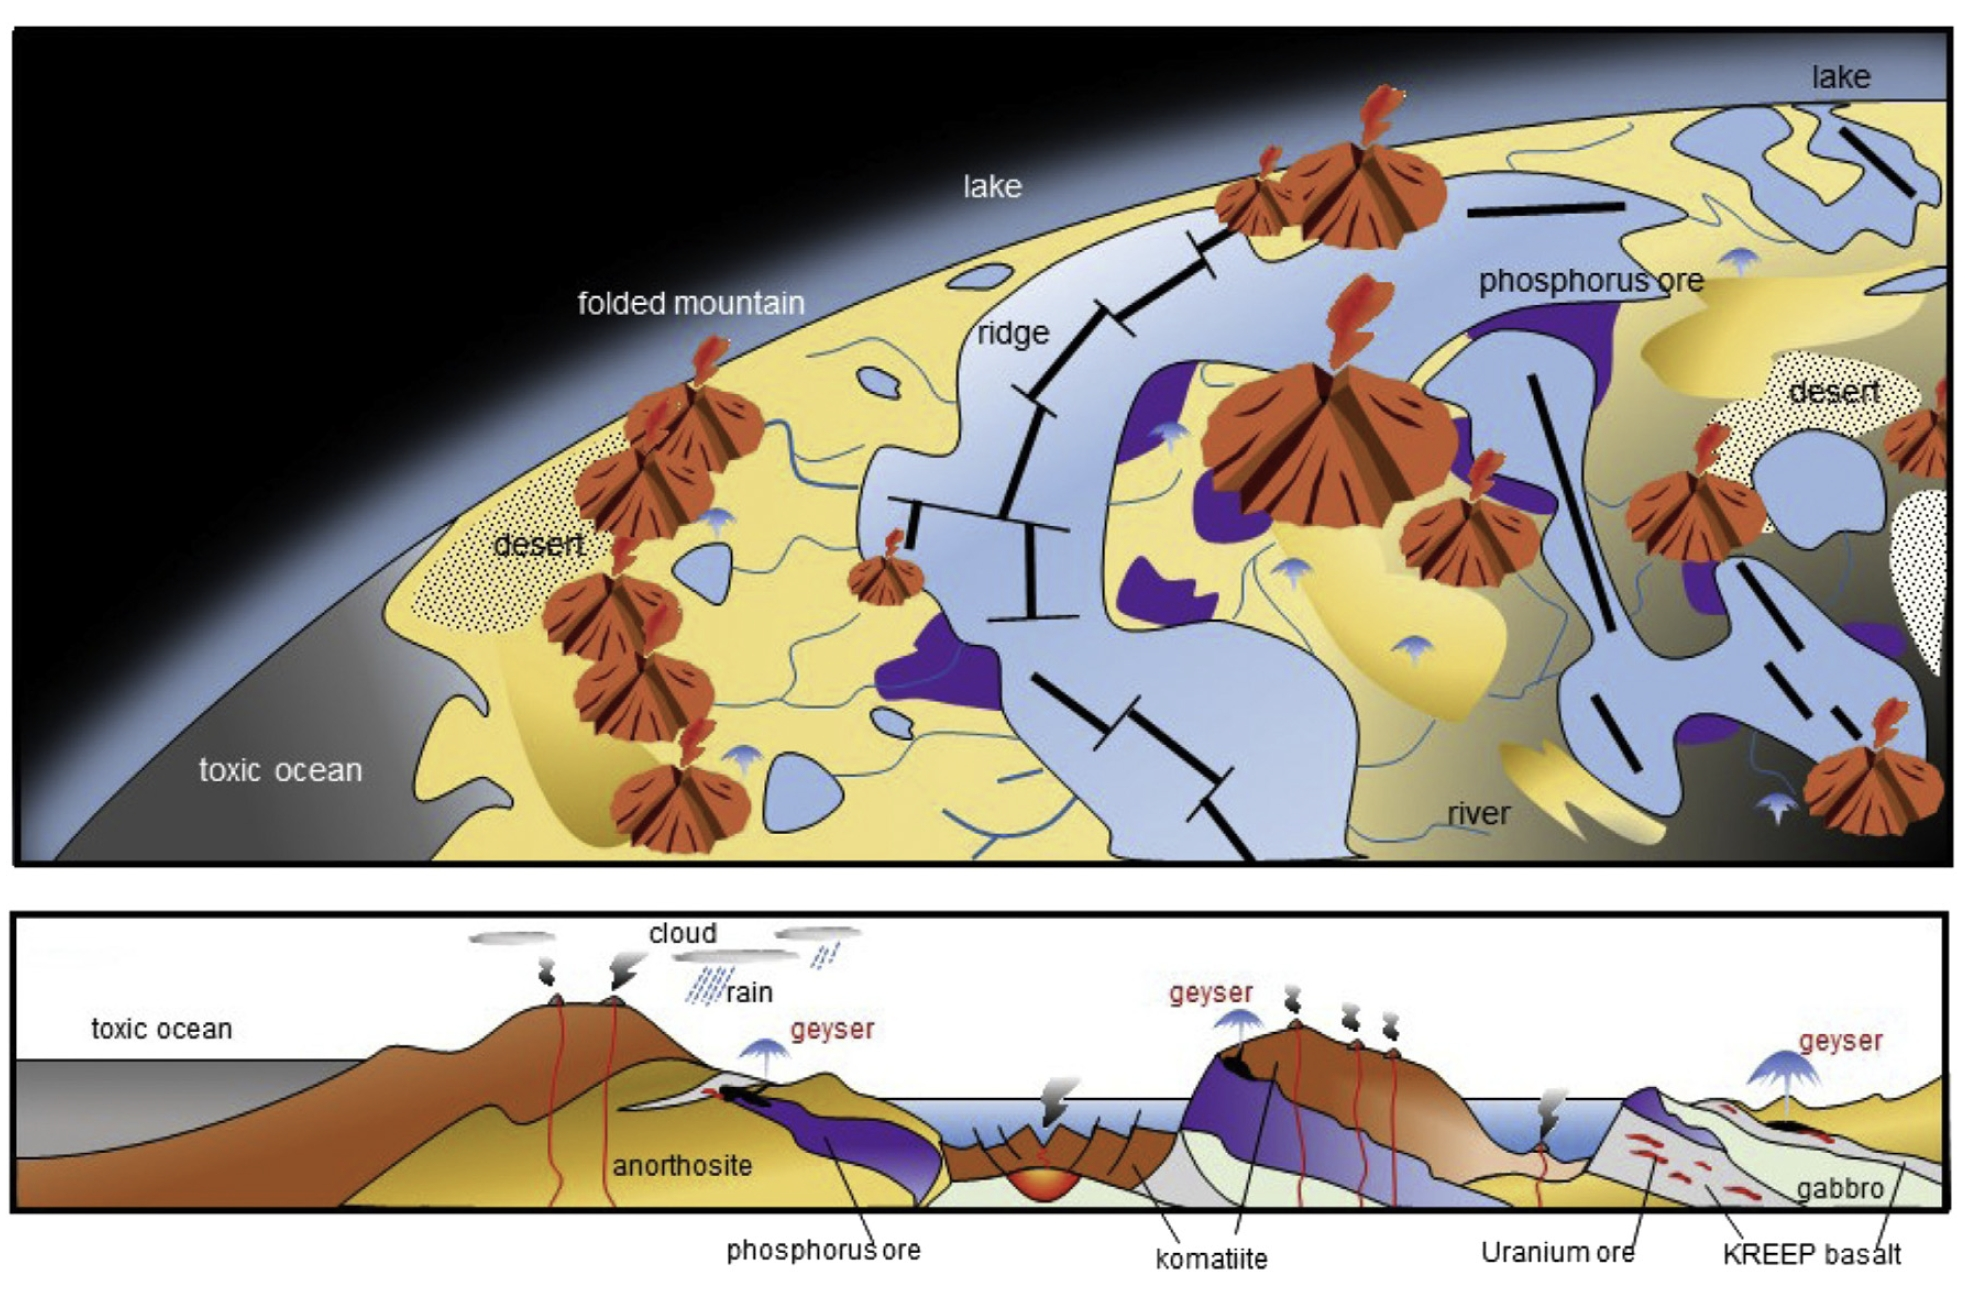
\includegraphics[width=0.9\textwidth]{GeochemicalLandscape}
\end{figure}

  
  \begin{itemize}
  	\item  Definitely an ocean that was warmer than today, probably saltier.\footnote{''While this is not my exact field of study, I am told that water-rock-atmosphere equilibriums operate at orders of magnitude faster time scales than planetary evolution. So the ocean “quickly” came to equilibrium with early oceans (maybe a million years or less), then as new rock was exposed, and the atmosphere changed, the equilibrium shifted. The composition may have been different, with more reduced metals for example, but sodium chloride is the most abundant ionic compound and likely always has been.''--Sarah Maurer}\cite{knauth1998salinity} 
  	\item Landmasses from volcanic activity, and, maybe, plate tectonics.
  	\item On continents, lakes and ponds from precipitation.  Maybe temporary streams from precipitation.
  	\item Surfaces composed of minerals, which were good for catalysis and energy production. Today covered with life.
  \end{itemize}


\subsection{Mixing processes between chemical reactors}
\begin{figure}[h!]
	\caption{Mixing processes between chemical reactors \cite{stueken2013did}}
	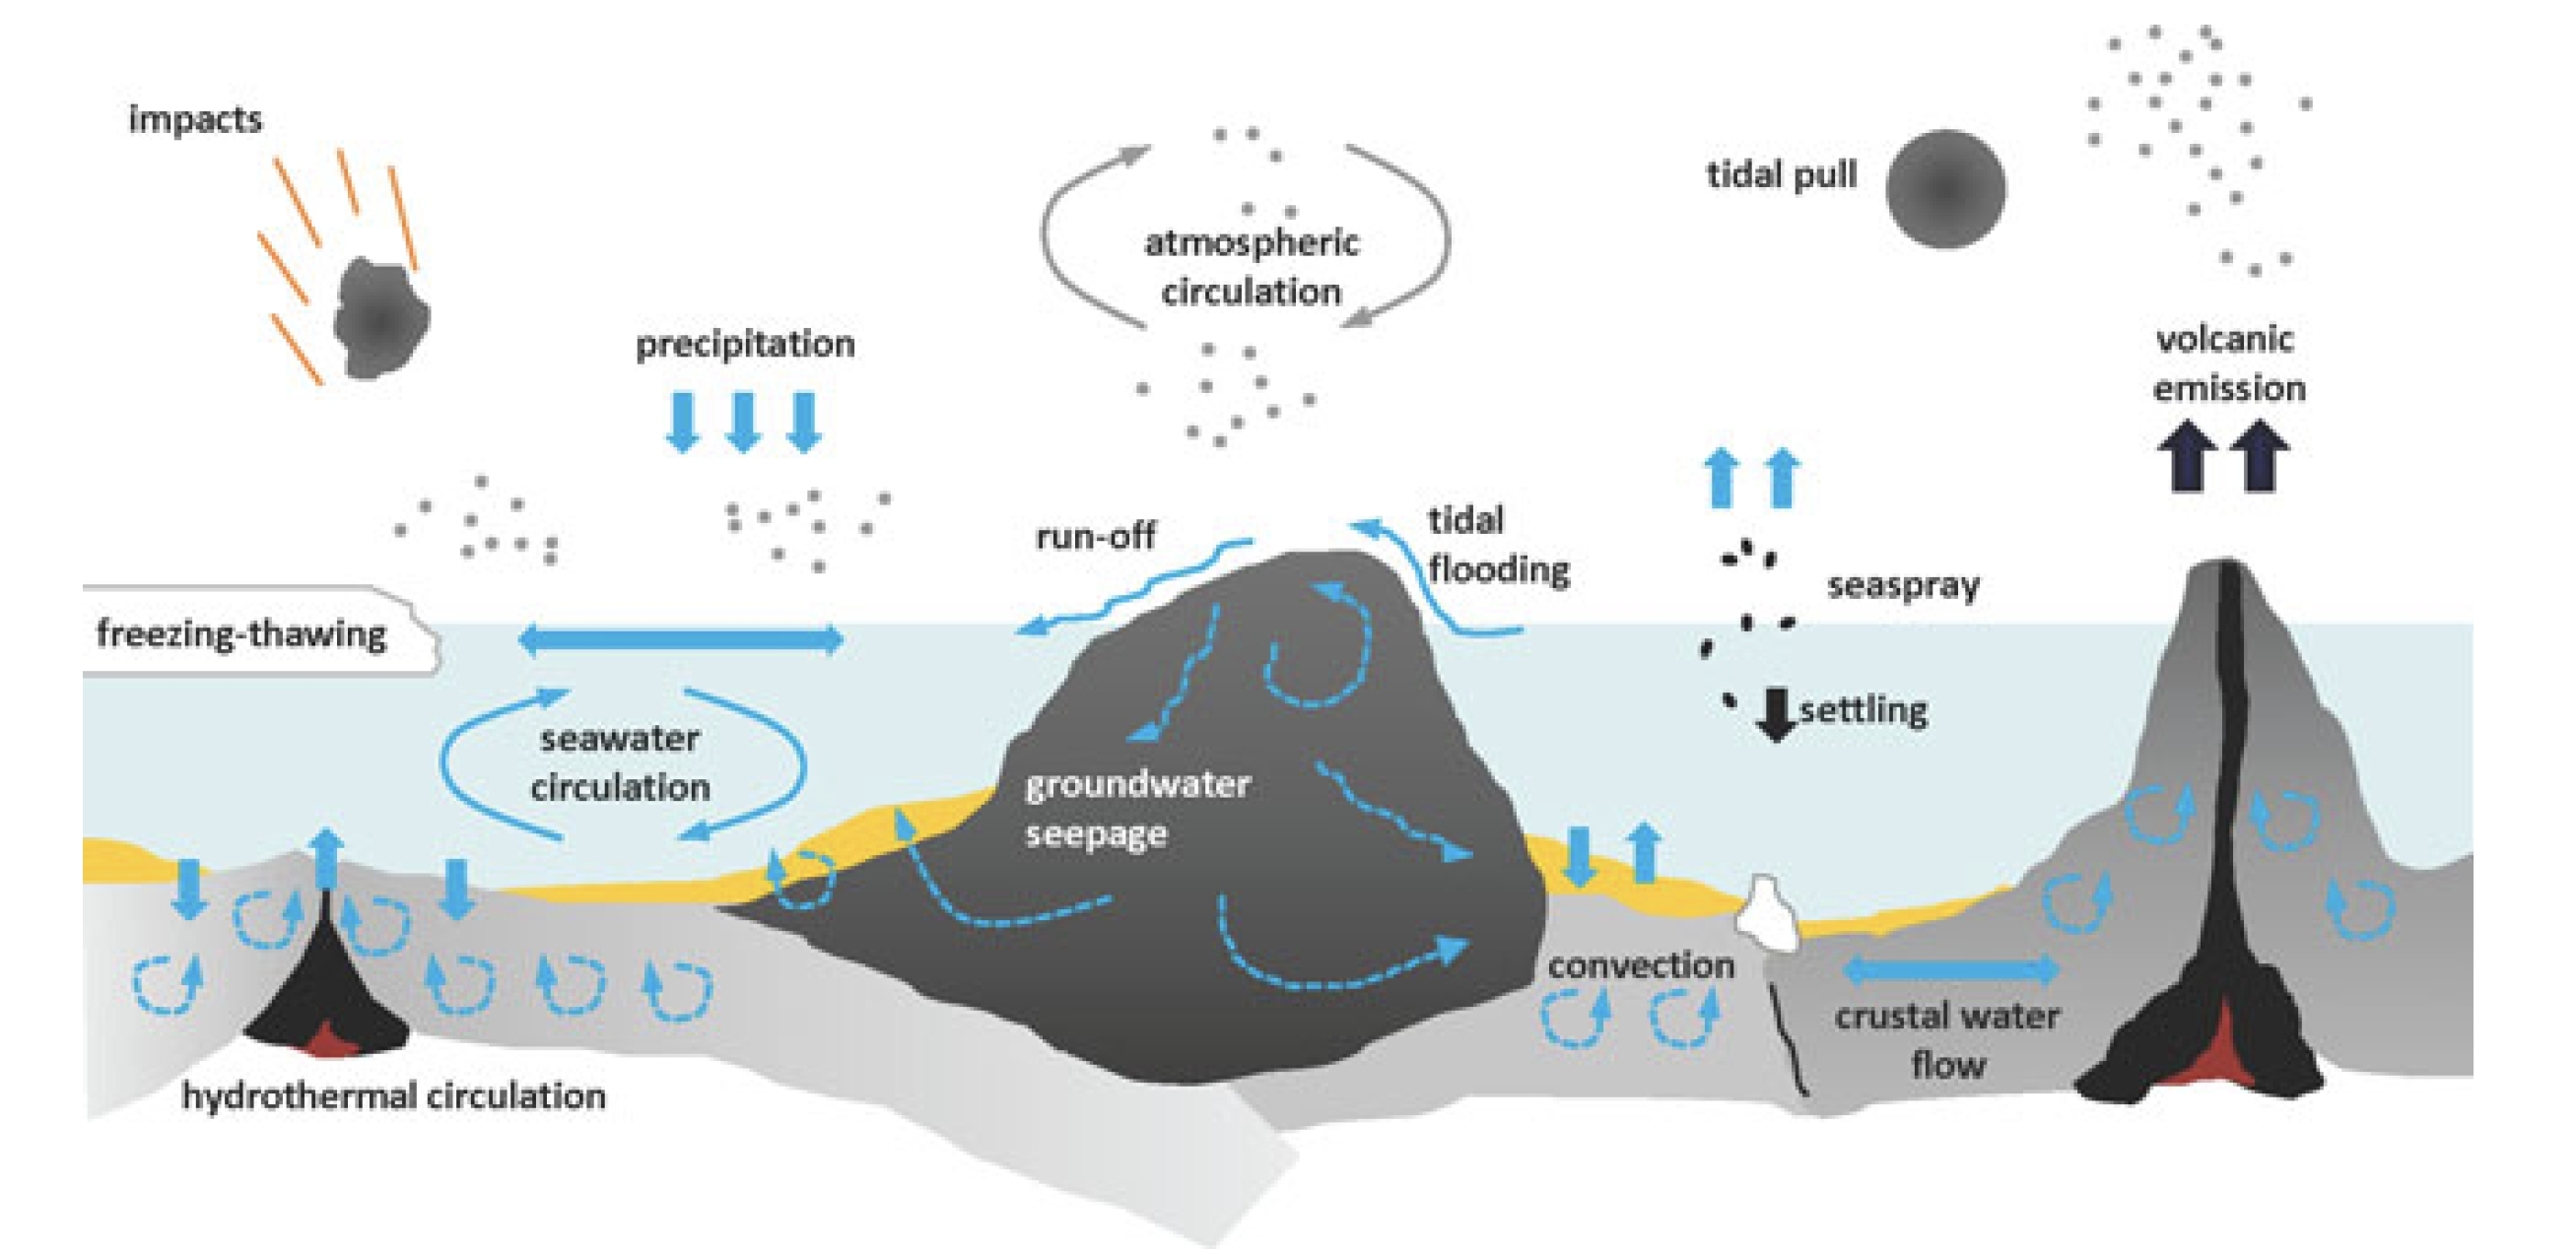
\includegraphics[width=0.9\textwidth]{MixingProcesses}
\end{figure}
Chemical reactions mixed by a variety of processes.

\begin{itemize}
	\item Tides
	\item Evaporation and aerosols
	\item Volcanic plumes
	\item Hydrothermal vents
\end{itemize}
  
  
\subsection{Geothermal systems}
\begin{figure}[h!]
	\caption{Geothermal systems \cite{damer2016field}}
	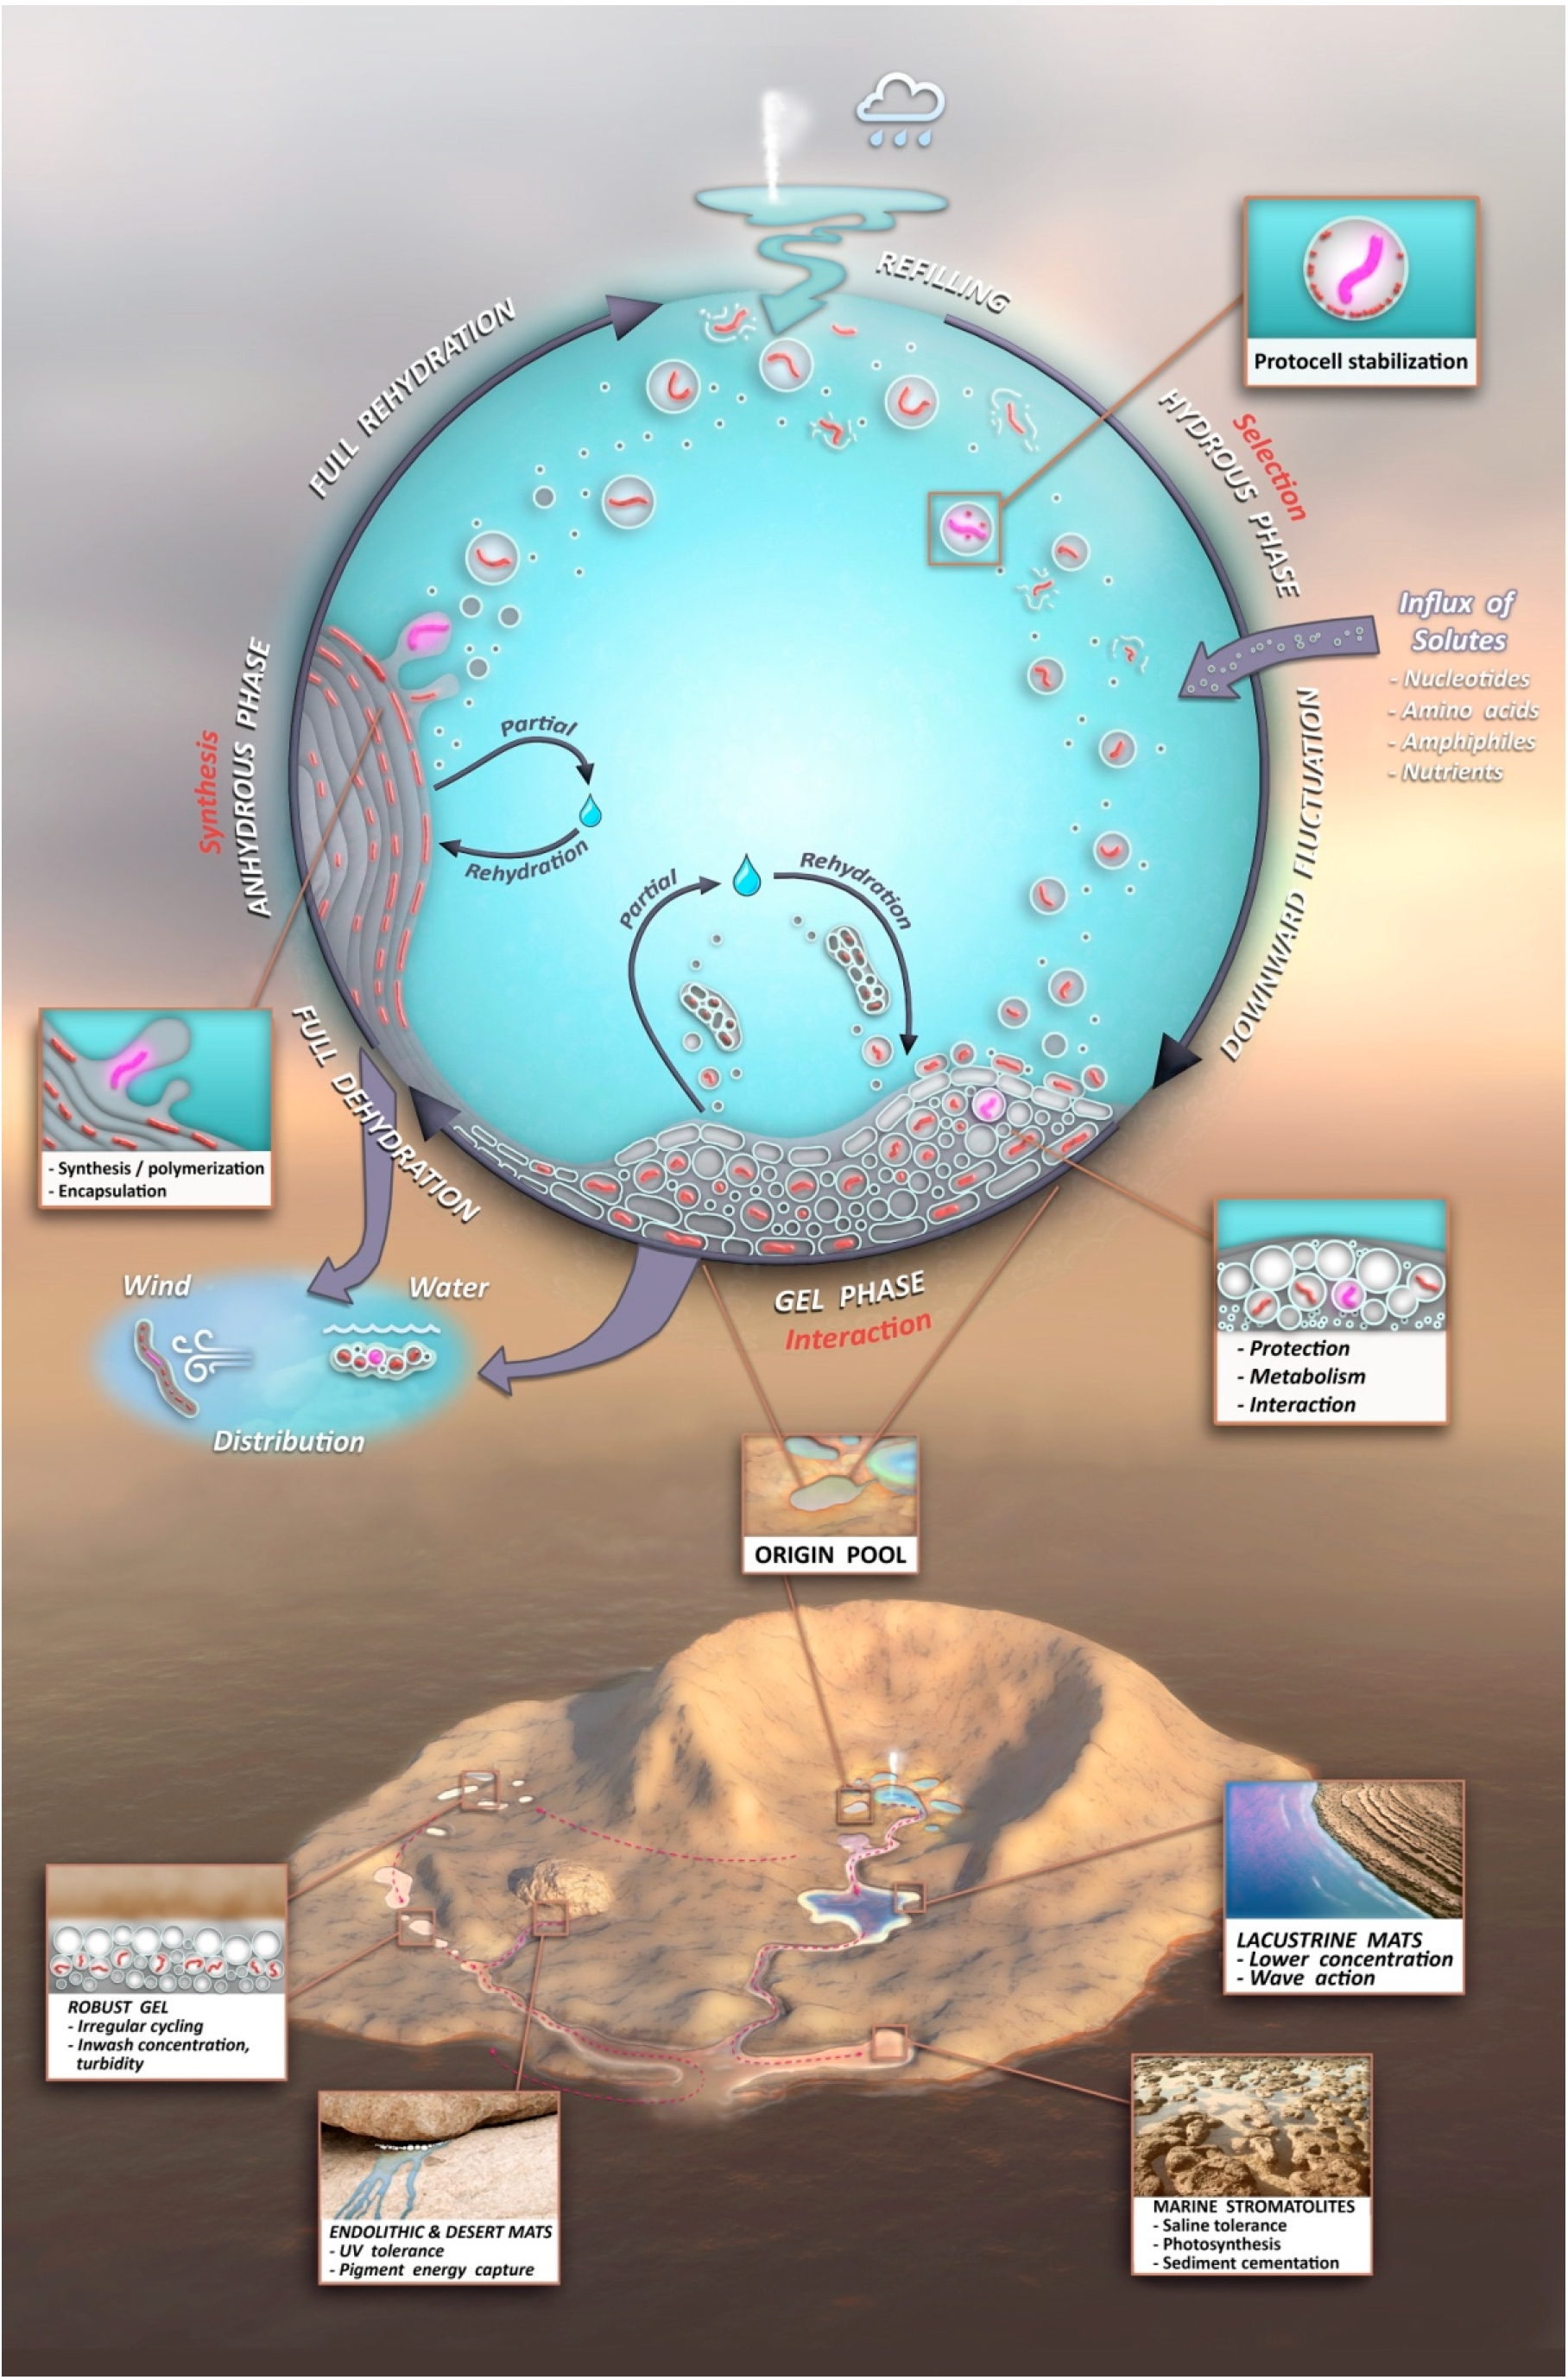
\includegraphics[width=0.9\textwidth]{GeothermalSystems}
\end{figure}

\begin{itemize}
	\item Provide high temperature, high pressure, reduced	reaction products
	\item Fresh water from 	precipitation
	\item Diversity of mineral	surfaces for ”nutrients” and catalysis
\end{itemize}

\subsection{Energy Sources}

See \cite{kitadai2018origins}, \cite{stueken2013did}, \cite{damer2016field}, \cite{miller1959organic}, \cite{ehrenfreund2002astrophysical},\cite{dalai2016incubating}, and \cite{chyba1997comets}.

\begin{itemize}
	\item Chemical Energy
	\begin{itemize}
		\item Reducing gases
		\item Radiation
		\item Minerals
	\end{itemize}
	\item Other Energy Sources
	\begin{itemize}
		\item Volcanic lightning
		\item UV-light
		\item High temperature
		\item Pressure
		\item Impacts
	\end{itemize}
\end{itemize}
Miller Urey. Maybe no methane, but CO2 to derive different mixture.

\begin{figure}[h!]
	\caption{Miller Urey \cite{miller1959organic}}
	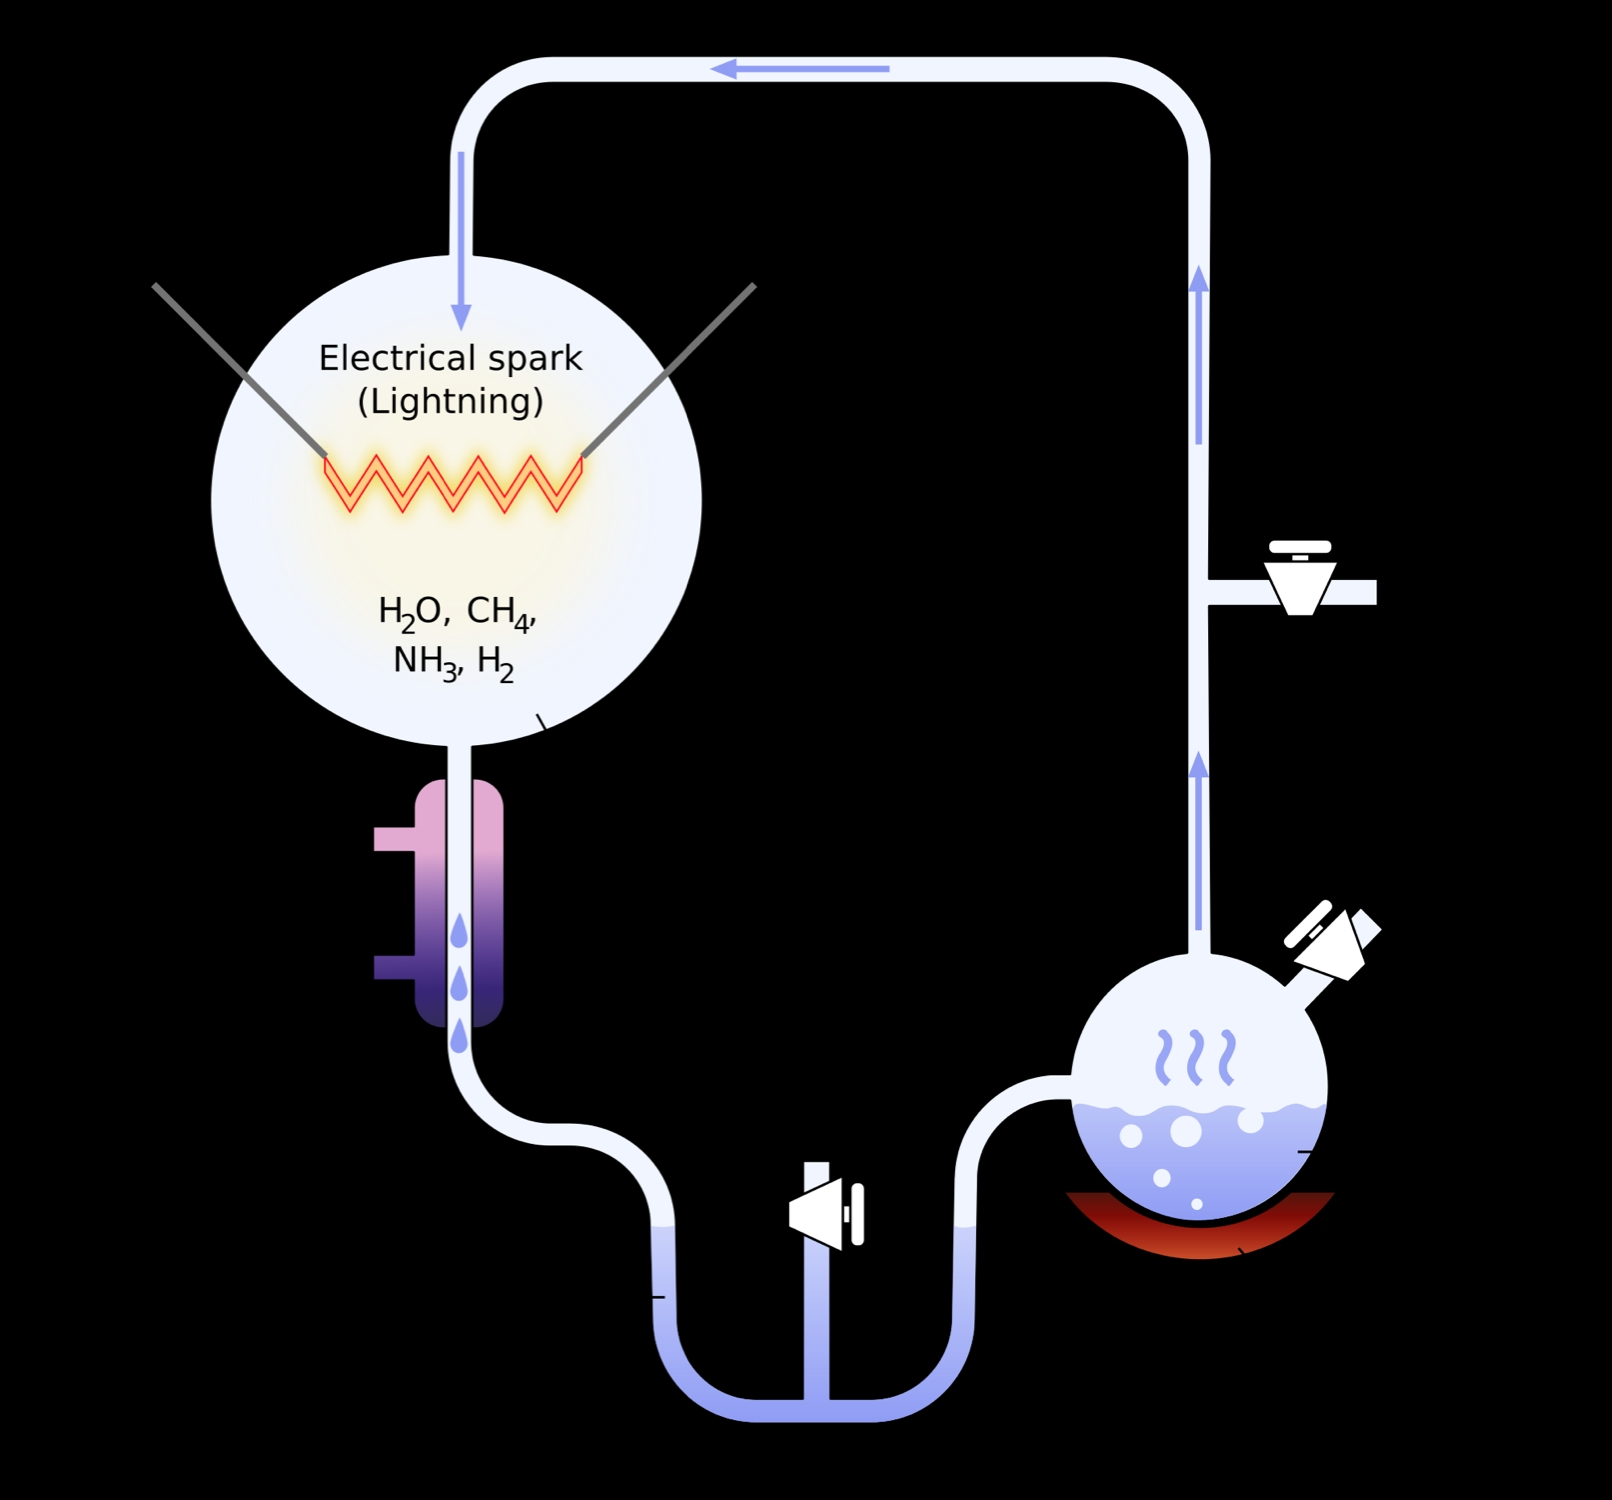
\includegraphics[width=0.45\textwidth]{MillerUrey1}
	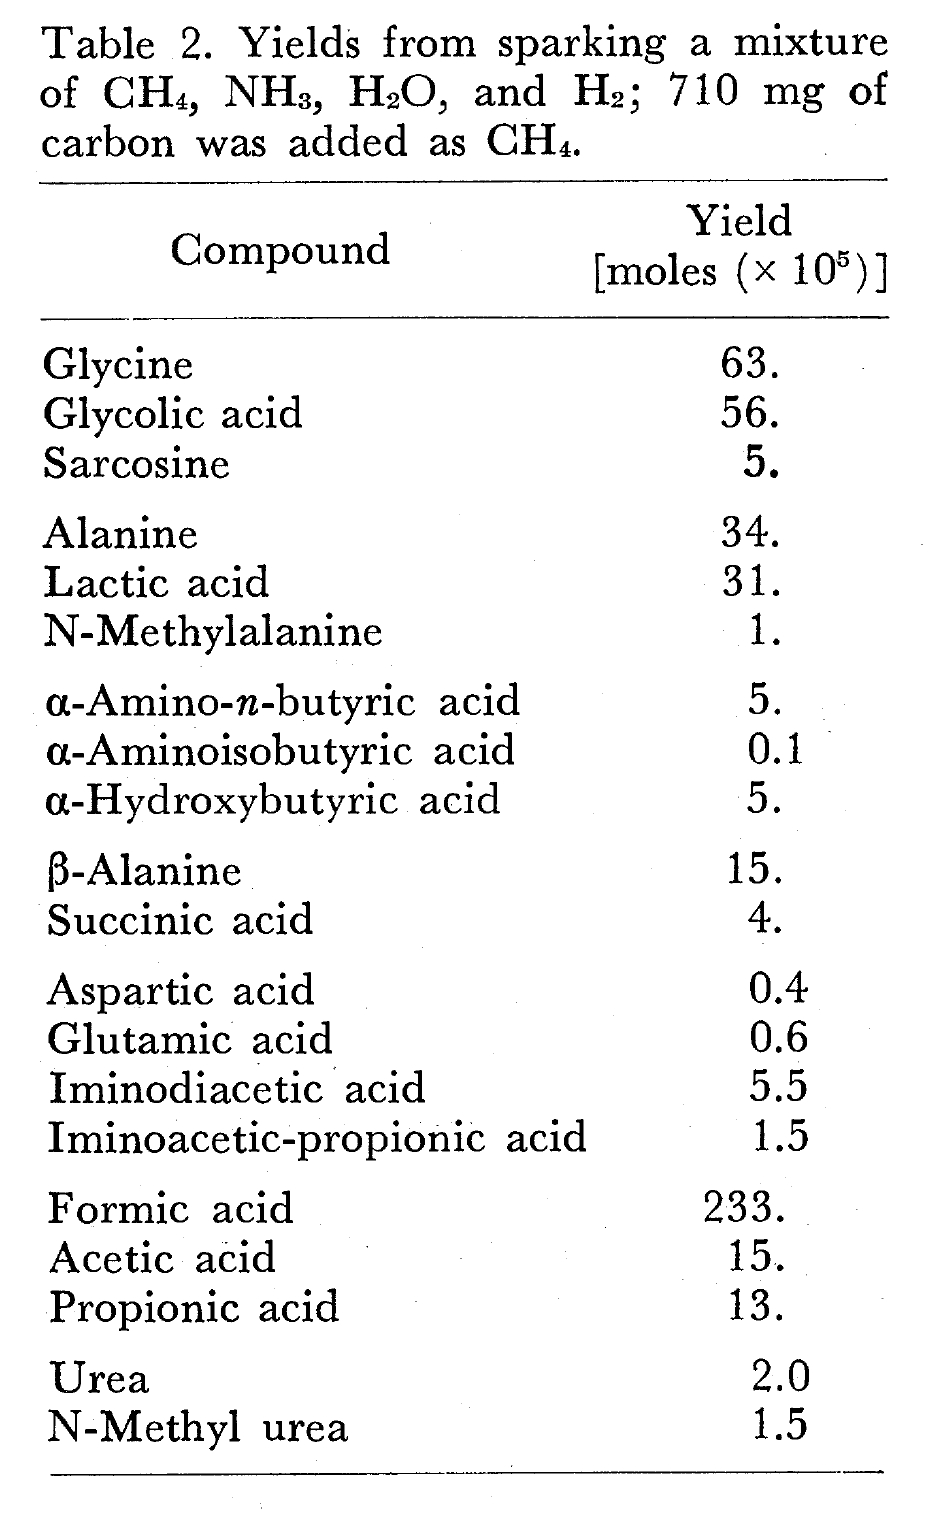
\includegraphics[width=0.45\textwidth]{MillerUrey2}
\end{figure}

Each meteorite has different chemical library

Enough material to jump start life

Bombardment

Samples and surface are (mostly) undisturbed
• Samples can be dated ( 40 Ar/ 39 Ar, 87 Rb/ 87 Sr, etc.)
• Craters can be counted
Lunar cratering rate anchors
the impact chronology for the
entire (inner) Solar System

Late Heavy Bombardment

\section{Likely Environments for Studying Origins of Life}

\begin{figure}[h!]
	\caption{Life probably started between 4.4 to 3.8 billion years ago (Ga) \cite{domagal2016astrobiology}}
	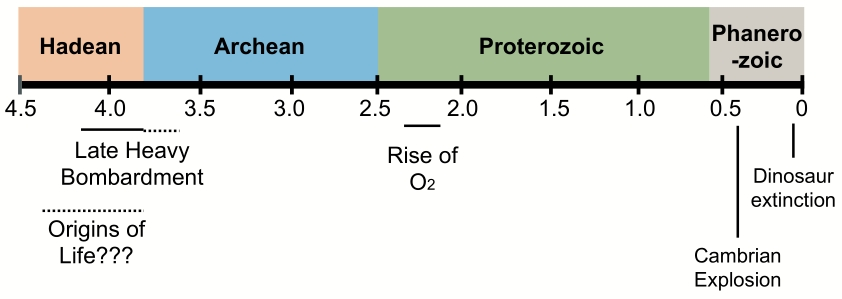
\includegraphics[width=0.9\textwidth]{LifeProbablyStarted}
\end{figure}

\begin{figure}[h!]
	\caption{Earth during the Hadean Eon was probably very inhospitable for life} 
	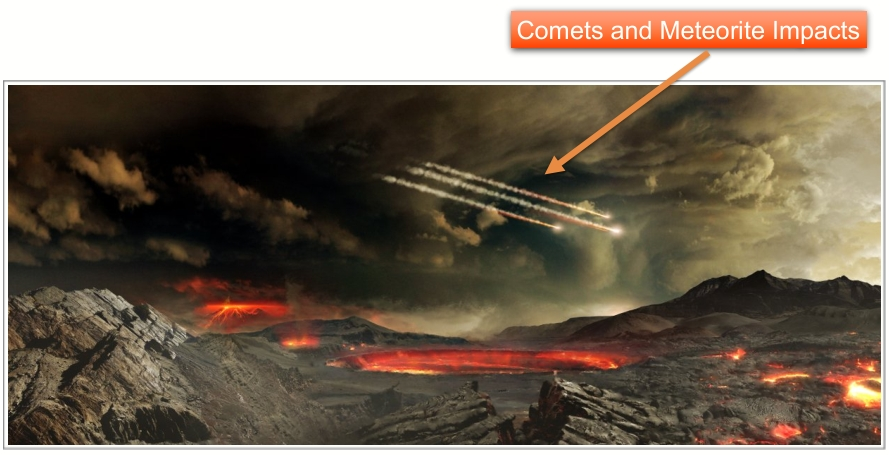
\includegraphics[width=0.9\textwidth]{HadeanInhospitable}
\end{figure}
 Magma Oceans formed because of:
\begin{itemize}
	\item Comets and meteorite impacts
	\item Tidal heating (moon/Earth)
	\item Core formation (plate tectonics)
\end{itemize}

Plate tectonics helped make the early Earth environment favorable for life

Global oceans probably covered the surface of the Earth by the Archean Eon

\begin{figure}[h!]
	\caption{Life took hold on Earth during the Archean Eon} 
	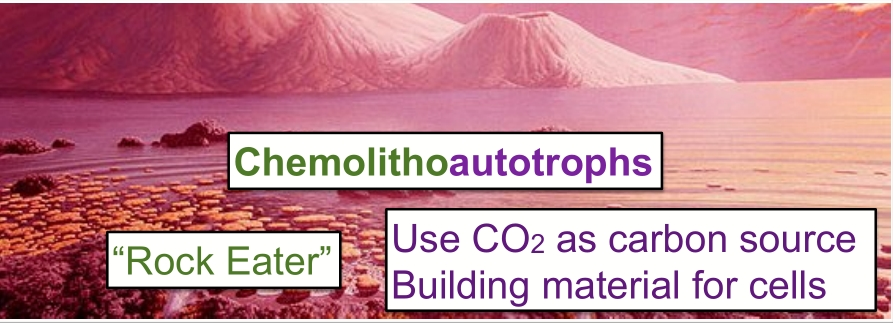
\includegraphics[width=0.9\textwidth]{Chemolithoautotrophs}
\end{figure}

The first likely signs of life in the rock record dates back to 3.5 to 3.3 Ga

\subsection{Cuatro Ci\'enegas Special Feature}

This is a short film about the people and places of the Cuatro Ci\'enegas Basin in Coahuila, M\'exico.\footnote{This is the transcript from the video, with a few small edits.} The Cuatro Ci\'enegas Basin - its water and microbial, plant and animal communities -
are a treasure of M\'exico. All of this unique life has been uncovered through the work of Mexican scientists with international collaborations. This work makes possible a deeper understanding of the history of all of life on earth.

\begin{figure}[h!]
	\caption{The Cuatro Ci\'enegas Basin} 
	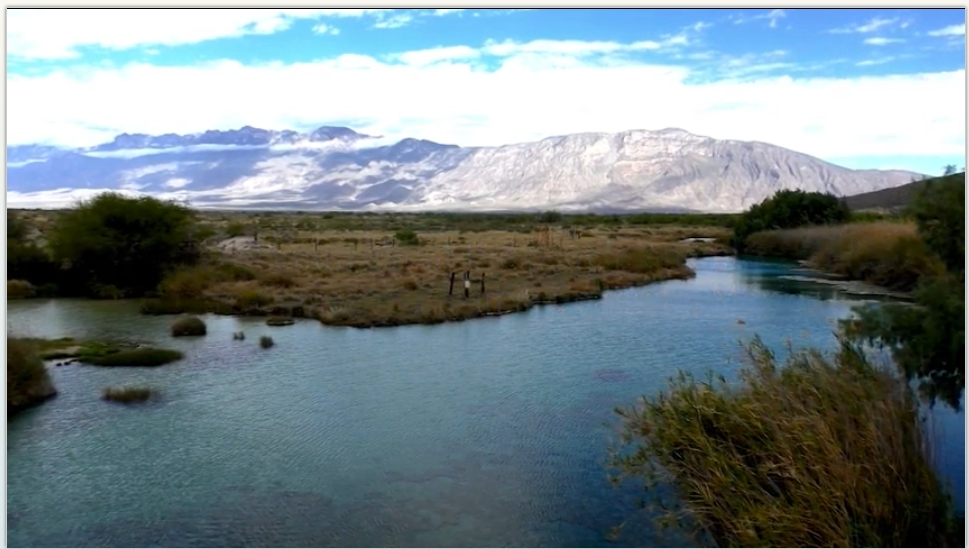
\includegraphics[width=0.9\textwidth]{CuatroCienegas1}
\end{figure}

My name is Valeria Souza. I work as a researcher at UNAM - the National University of Mexico, that is a very large university. This is probably the most important site
that we have in the world right now to understand the origin of diversity. This place has an amazing geology that you can see just in front of you.\cite{souza2018lost}

\begin{figure}[h!]
	\caption{We have that kind of tsunami of rocks} 
	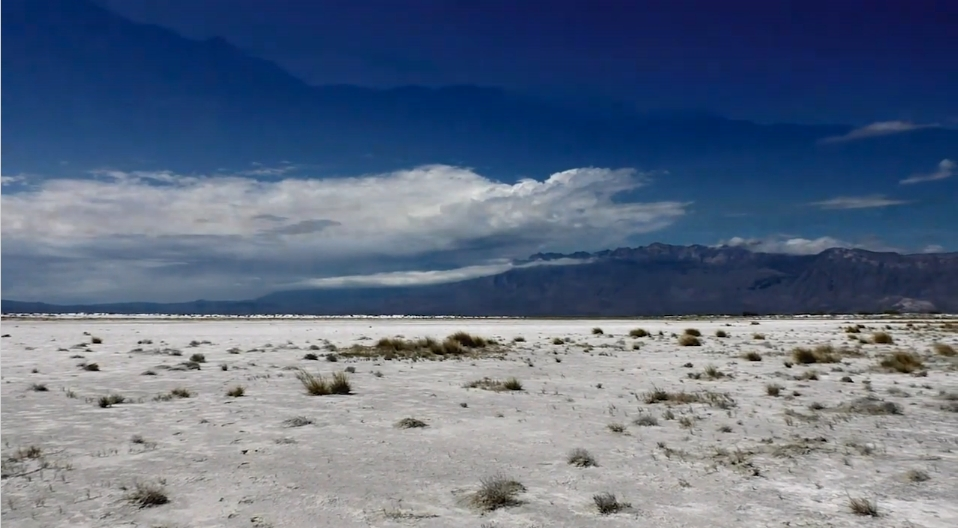
\includegraphics[width=0.9\textwidth]{CuatroCienegas2}
\end{figure}

We have that kind of tsunami of rocks that uplifted, because the mountain
that is over that edge is like an arrow. It has an active fault
with magma underneath. And, it's pushing all the marine sediments that are from this valley up and then it's flipped and makes a heart shape -- a 3,000 meter mountain.

So, all this amazing geology is an explanation of why Cuatro  Ci\'enegas is a singularity -- because these marine sediments store the conditions of the ancient sea. They store the magma that is rich in sulfur, that takes us all the way back to the Archean, and it stores the minerals that formed in sand. These minerals are very old.

Also, it is a sediment that is devoid of the most basic element for life, that is, phosphorus. So, this site is amazingly poor in phosphorus, and that makes for a very
skewed stoichiometry. Most of life now cannot live in a skewed stoichiometry -- we need 60 nitrogens for each phosphorus. Here, we have 100 nitrogens - at least - for each phosphorus, in some places 200 nitrogens for each phosphorus.

So, how they can make basic things, such as ribosomes or DNA, is because they are really good at stealing phosphorus from anybody else, including rocks. So, they have an amazing array of strategies to deal with the lack of phosphorus, and they did that since the Archean.

So, here we have stromatolites and microbial mats, whose ancestry goes back
to the Precambrian in some cases. And, we are going to a site where we think we have the boundary between the Archean and the Precambrian\footnote{Should this be Proterozoic?}. Since this is a blue pool, we are talking about the moment where animals turned the planet blue, and that was in the Ediacaran in the late Precambrian.

My name is Maria Kalambokidis, and I'm an intern for a year, working in Valeria's lab in UNAM, in the Department of Evolutionary Ecology. And, right now, we're at Pozas Azules, at the site of the Archaean domes. 

\begin{figure}[h!]
	\caption{A microbial mat that created a bubble through the activity of the methanogens} 
	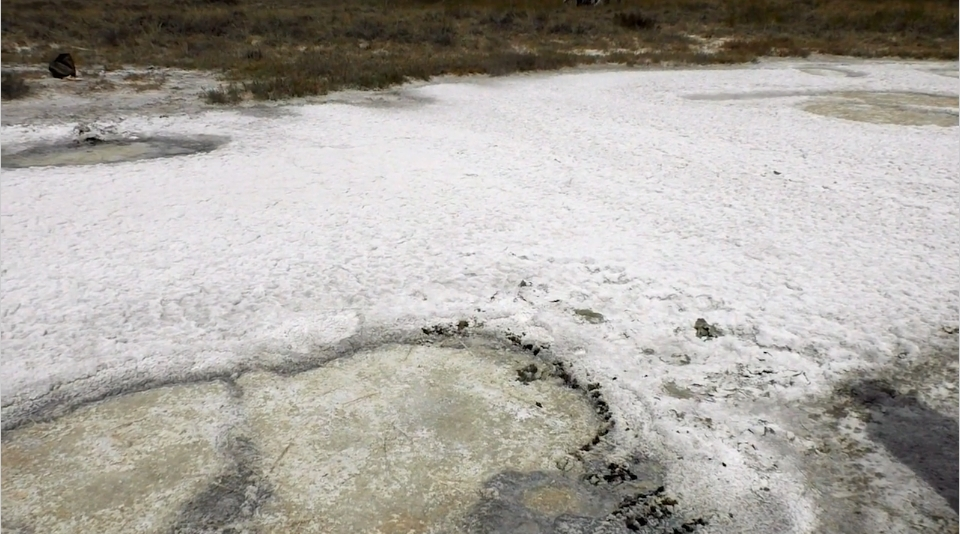
\includegraphics[width=0.9\textwidth]{CuatroCienegas3}
\end{figure}

So, here you have a microbial mat that created a bubble through the activity of the methanogens. It created a bubble and then it eventually burst, creating this perimeter. So, we sampled the microbial mats that are still present there. And, right now, they're hidden beneath the salt crust, because it's so dry. My research is looking at the evolutionary resilience of the microbial mats at Cuatro i\'enegas.

So, the microbial mats create a codependent community where each layer is sort of representing the history of metabolisms on Earth. So, you start with methanogens, 
which create nutrients for the next layer of sulfur-oxidizing bacteria, all the way up until photosynthesis. So, through this community, they've become really dependent on each other and they evolve together, creating a really resilient community in Cuatro  Ci\'enegas that has existed for many millennia.

I was interested in the microbial mats because they're evolutionary resilient
and they've existed so long here, but also because they've existed in an environment that many other organisms couldn't exist. For example, a really low nutrient content, in particular, low in phosphorus, which is thought to be necessary for the building blocks of life.

So, they've existed for so long, they're able to exist in extreme environments. Therefore, it creates a sort of living laboratory of organisms that are alive today and indicative of communities that existed long ago. So, in origin of life research and in astrobiology, usually you're looking for signs of life - like biosignatures on another planet, or you're breaking open old rocks to see if there are compounds indicative of life. But, in Cuatro  Ci\'enegas, and in these mats, we think that we have the organisms that formed the same communities that existed long ago.  So, as a biologist, it's really exciting to actually be able to study it alive today.

The big questions why so many species on planet Earth or in this place
???the history of survival???

The origin of life was probably very easy.

The origin of life was probably ??????
millions of ways possible???

On this planet, life survived???

???? the rocks
and transformed all of the minerals.???

My name is Gabriela Olmedo-Álvarez, and I work at Cinvestav: ''center of research for advanced studies.'' I'm in Mexico, right in the middle of Mexico - in Irapuato. I'm the director of Cinvestav in Irapuato, although I am also a researcher. And, I've been working for 15 years, close to Valeria Souza, in trying to decipher what are the keys that allow so much diversity of microorganisms inhabit these places.

\begin{figure}[h!]
	\caption{Pond with few nutrients but plenty of life.} 
	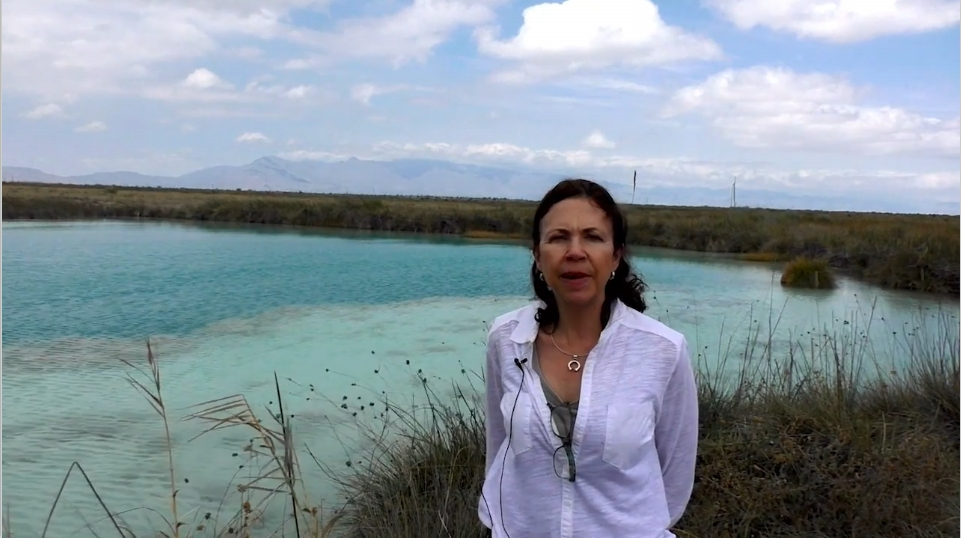
\includegraphics[width=0.9\textwidth]{CuatroCienegas4}
\end{figure}

And, if you are looking at the pond behind me - that's a beautiful pond, and it looks like it doesn't have much, because it doesn't have a lot of nutrients. That is why it's so interesting - it doesn't have nutrients, but it has lots of different bacteria, and has evidence of very old life.

It also has these stone-like things that are stromatolites. Stromatolites are evidence of the first types of life on the planet, but here they are still alive. They are still, you know, blooming, and it's very interesting because these are very, very old types of life. And, that is possible precisely because there are no nutrients. So, other larger things
cannot compete with it, and that allows these to remain for centuries and millions of years.


But if we walk just a few meters away, maybe just 200 meters, we'll find a very different scenery. We'll find these very salty crusts, and these salty crusts are full of life also - a very special life with lots of salt and with a low pH. So, it's a weird life that we do not understand, and that's sort of one of the focuses that we have for this trip - to be able to sample what things are living there. And, we'll take them to the lab to figure out how some bacteria or archaea can live with these very, very extreme environments.

\begin{figure}[h!]
	\caption{These salty crusts are full of life also - a very special life with lots of salt and with a low pH.} 
	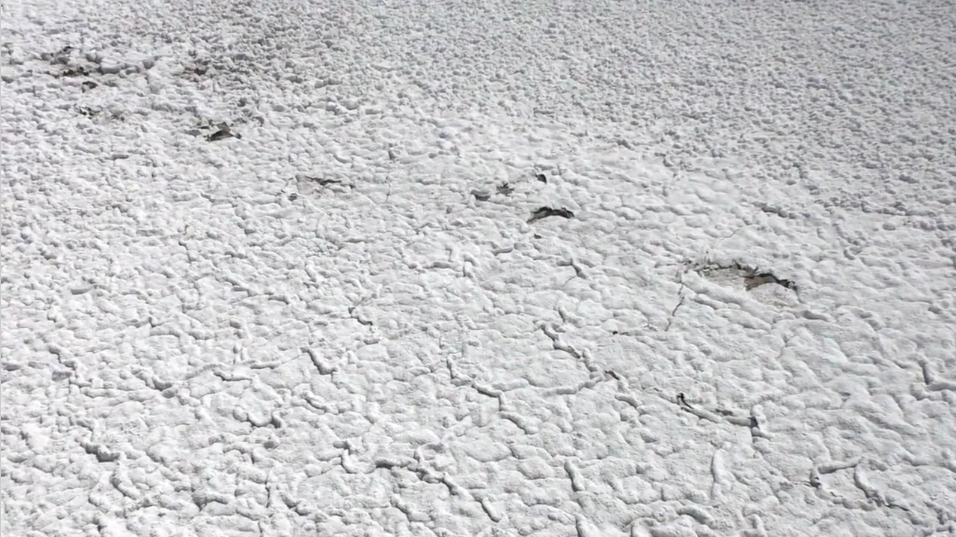
\includegraphics[width=0.9\textwidth]{CuatroCienegas5}
\end{figure}

In the system called ''Pozas Rojas'', because these ponds are fluctuating environments, they get very saline in the summer because the water evaporates. It is deep water, not rain water, so each one becomes a more vivid color than in winter, where water doesn't evaporate as much -- so they get like the juiciness concentrated in the summer.

The life that lives here is very diverse - there's microbial mass that we have sequenced. There's a very large biodiversity and there are like islands. There are nine small islands of these tiny \gls{gls:poza}s and a big lagoon. So, you can compare the diversity in each one of them separately and then the big \gls{gls:poza} in the middle. But, this was perturbed by a hurricane in 2010 and it became a complete lake, all of its... It kind of drained all the nutrients and all the water from the... east side of the valley. The biology changed because the \gls{gls:poza}s became connected 
with the lake water, and also the nutrients changed. It was - before the hurricane - it was the site with less phosphorus. Now, it is a site that nearly has a balance of stoichiometry. So, it is very interesting how the life got habituated to this richer environment. What is even more interesting is that what was a very primitive site it became a more Holocene site.
\begin{figure}[h!]
	\caption{The life that lives here is very diverse - there's microbial mass that we have sequenced.} 
	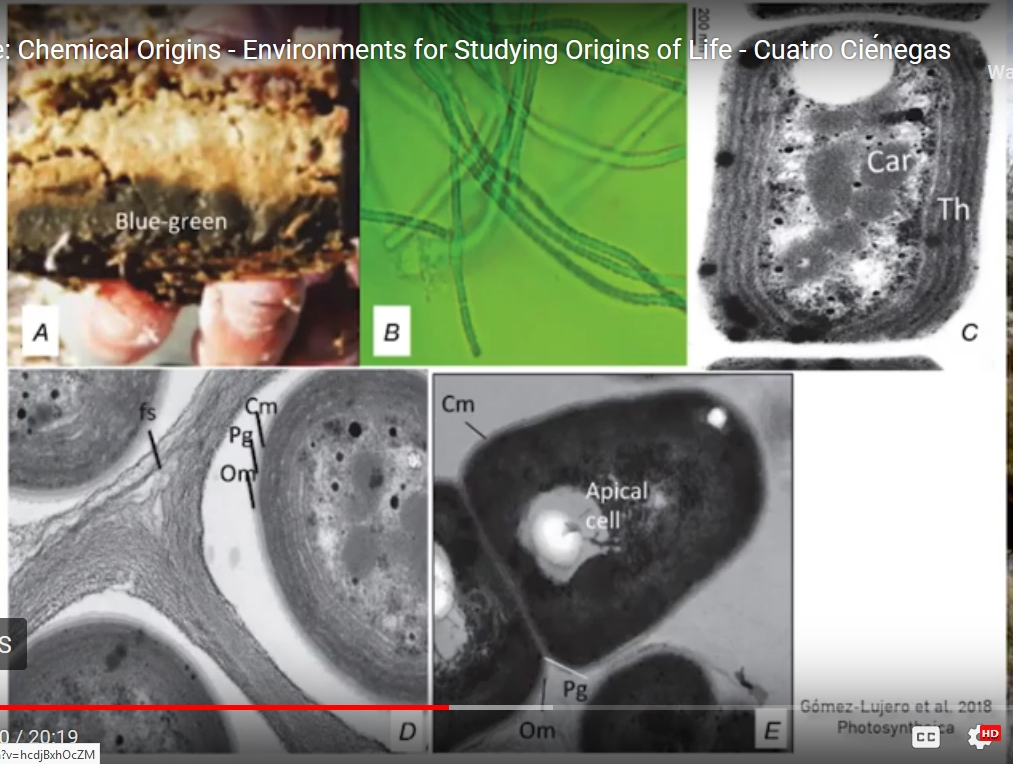
\includegraphics[width=0.9\textwidth]{CuatroCienegas6}
\end{figure}

\begin{figure}[h!]
	\caption{There are nine small islands of these tiny \gls{gls:poza}s and a big lagoon.} 
	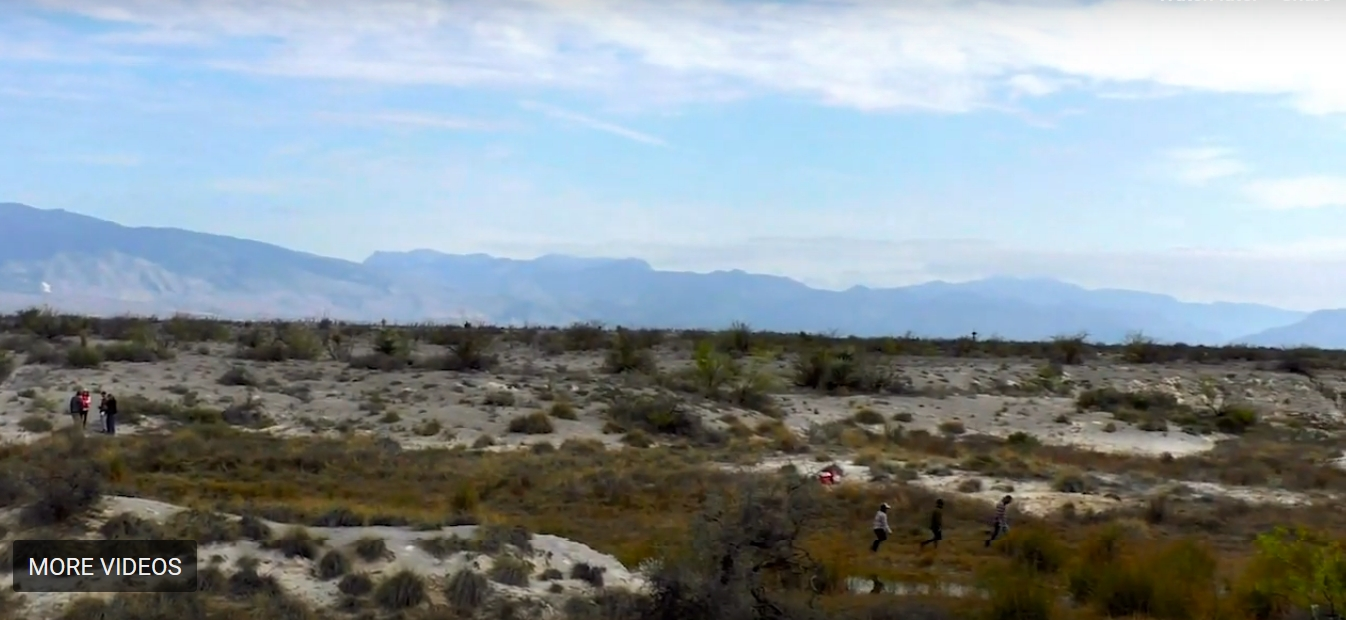
\includegraphics[width=0.9\textwidth]{CuatroCienegas7}
\end{figure}

For example, the Vibrio that lives here, they didn't radiate since the Holocene in Cuatro  Ci\'enegas, which is at the same time as the fishes came from the R\`io Bravo shelf. So, they are very interesting, and they are always changing, and that makes us really happy --and we are following their change. So, I'm sure that the deep aquifer still has the deep, ancient bacteria. It shows that the lake that shaped here, that came here, brought newer creatures from everywhere that were bacteria more used to nutrients. And, maybe there are pockets of nutrients in different parts of the valley.

What makes Cuatro  Ci\'enegas unique is precisely the lack of nutrients. Maybe they are going to become - each time that we sample - more and more imbalanced and return to their ancient selves. But, it will take time.

My name is Jorge Valdivia, and I am a full-time professor at the Universidad Nacional Aut\'onoma de M\'exico. [...] of my doctoral studies in the Cuatro  Ci\'enegas valley. I was working with the genus Bacillus and the project was focused on knowing the relationship that existed between the number of copies of the ribosomal operon and with the available phosphorus.\cite{valdivia2016variability}
\begin{figure}[h!]
	\caption{Variability of the rRNA operon copy number in the Bacillus diversity from the Cuatro  Ci\'enegas basin} 
	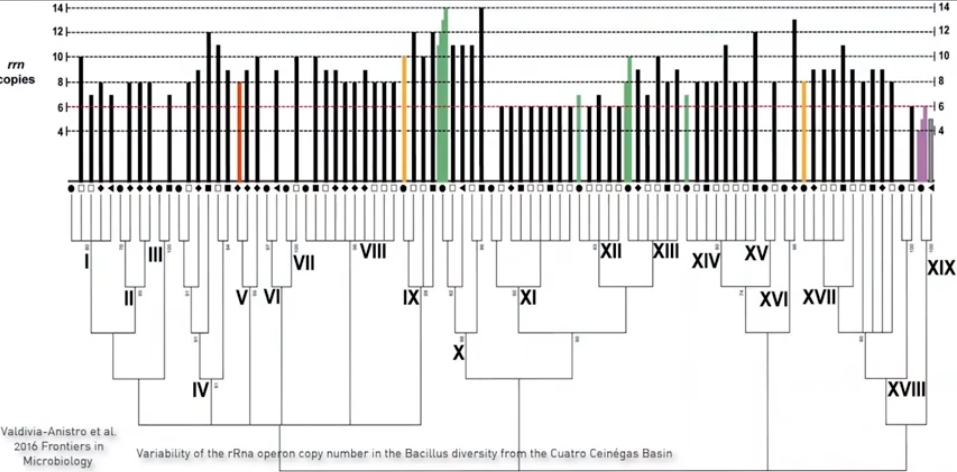
\includegraphics[width=0.9\textwidth]{CuatroCienegas8}
\end{figure}

It is known that the valley of Cuatro  Ci\'enegas is an extremely \gls{gls:oligotroph}ic site. With these conditions...they are homologous to what... the conditions in the past [...] origin of life. Then, the interesting thing to find out was how a genus that is characterized by having many copies of the ribosomal operon can adapt to these conditions of extreme oligotrophy.

We wanted to work in the isolates of the main sites in the valley, and we wanted to quantify the genome level - how many ribosomal operons they had. We set them to grow
with water from the site to replicate the natural conditions in which they are found living, and what we observe is that there is a zero correlation with respect to the hypothesis of the growth rate.

A good indication are the viruses. Viruses are the most ferocious hunters in the world. And, like ferocious hunters, each one has their own favorite prey. And, Cuatro  Ci\'enegas is the most diverse place on the planet for viruses at the tiniest scale. And, the favorite food of those viruses are bacteria

My name is Nahui Medina, and right now I'm a PhD student in Nuevo Le\'on in Monterrey. So, right now I'm doing this amazing project about Archaeas and extremophiles. What we do right now is try to isolate every single microorganism that we can, and we do this with amazing people in the lab, trying to create strategies to make these microorganisms live in the lab. This is pretty much interesting because Archaeas, you know, in Ancient Greek, is about "ancient," you know. This means that it could help us to know how they lived and try to understand...how life is...what begun... at that moment...it's pretty interesting...

They are so beautiful because they have so many colors - red, pink, and like a... yellowish, some of them. So, it's a pretty amazing project we're doing right now. 
Maybe because it's in a place where the whole ecosystem, and the whole habitat is 
it's not in another place, you know... you cannot find... the species that are in here. So, it's very... interesting because the microorganisms or the prokaryotes are living here. There's just living here and that's it. You cannot find them in another place in the world. So, that's what we're doing and we're so happy to do it.

\begin{figure}[h!]
	\caption{\Gls{gls:poza} Azul Two} 
	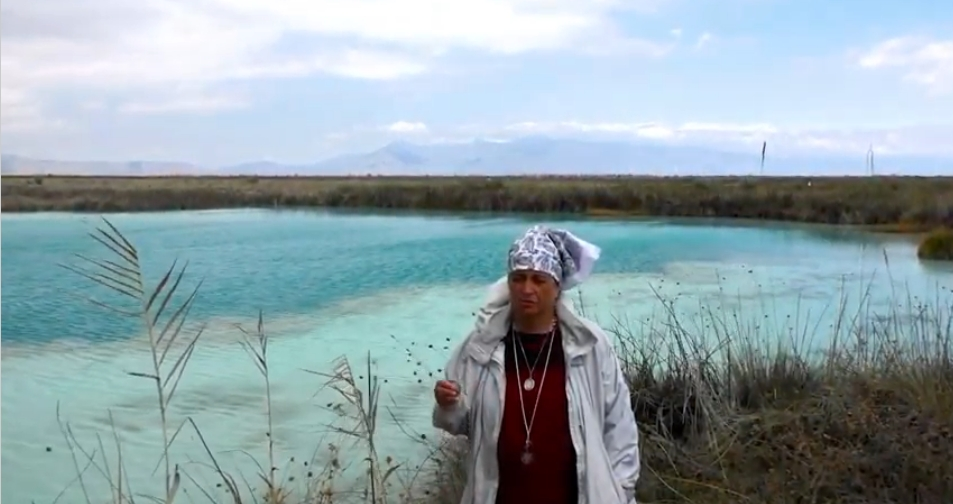
\includegraphics[width=0.9\textwidth]{CuatroCienegas9}
\end{figure}

Here we are in \Gls{gls:poza} Azul Two, that is one of the most beautiful \gls{gls:poza}s in all the valley. What we can see behind us is a very big stromatolite shelf. So, these blue \gls{gls:poza}s take us back to 600 million years ago when the animals changed the chemistry of the ocean and the ocean turned blue --and that's called the Ediacaran Era. So, in Cuatro  Ci\'enegas, we have kind of different timeframes - different moments in geology that got preserved. And, that's really interesting because it's not just a metaphor, it's not just that it looks like the Ediacaran, and when the ocean turned blue, and still the stromatolite shelf were being eaten by the first herbivores -- that was their doom.

\begin{figure}[h!]
	\caption{In the Archaean domes that are 50 metres over there} 
	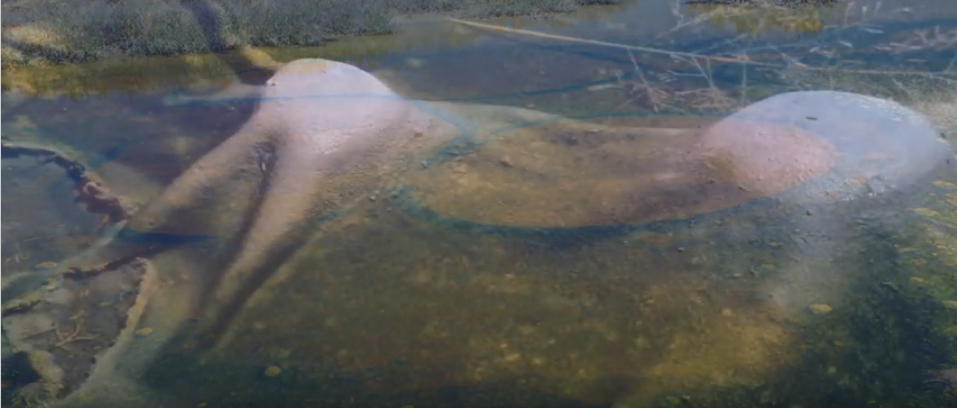
\includegraphics[width=0.9\textwidth]{CuatroCienegas10}
\end{figure}
But also, it's that this lineage has survived - survived for the longest time. In the Archaean domes that are 50 metres over there, we have evidence that the Archaean - a world of methane and CO2 - is preserved inside domes that are built by bacteria that protect the ancient anaerobic bacteria from the oxygen input, while they are doing photosynthesis. This kind of cooperation and construction of the whole niche is pretty unique. We know that stromatolite were world-builders - they made the ocean blue, they transformed every element that came from the start and made life complex. For the fact is that, here in Cuatro  Ci\'enegas, we have a window - a true window - of those lost worlds is really incredible.

Because you walk... meters and you find three billion years... of time. And, you can have lineages that are very, very divergent from the ones we know now, how they assemble their nutrients and how they work. We can cultivate them, we can study them using metagenomics. But, for them to be studied, we need water. And, this water here is precious -it's not just any water. So, water that comes from that mountain that has a magmatic heart, that magmatic heart is responsible for the Jurassic. So, what happened is - humans - we are really silly, and we think we can manage nature. When there's agriculture in the desert... where the water comes comes from -the deep aquifer. And, it is not just any aquifer - it's an aquifer that has stored the conditions of the early sea, and we are losing it.

\begin{figure}[h!]
	\caption{Then we have the tragedy of Churince where there's no longer water} 
	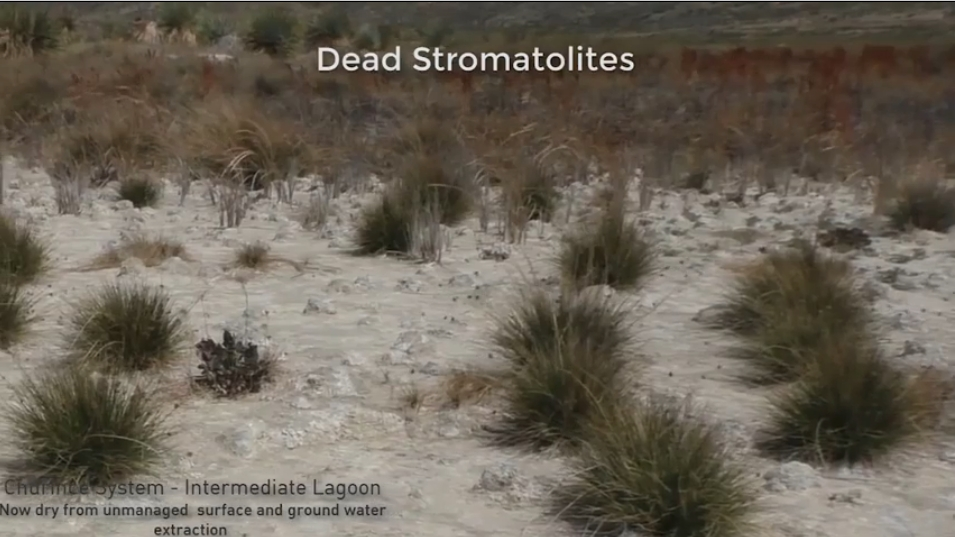
\includegraphics[width=0.9\textwidth]{CuatroCienegas11}
\end{figure}

Then we have the tragedy of Churince where there's no longer water. It only looks like that. And now, it's a field of dead turtles and dead fishes. Maybe there's some hope that we can recover it if we close all the channels that are taking out the water from this ecosystem.

See also \cite{gomez2018leptolyngbya} and \cite{taboada2018geographic}.

\section{Chemistry and The Origins of Life}

Tar problem: Biomolecules plus heat and time $\rightarrow$ black sludge.

\begin{itemize}
	\item What molecules can be and are created without life?
	\item How can these molecules be made to react in a life like manner?
	\item How can formation of wasteful byproducts like	tars be prevented?
\end{itemize}
\section{Why Nature Chose Phosphates}

\begin{itemize}
	\item Structural
	\begin{itemize}
		\item Nucleic Acid Backbones (Figure \ref{fig:PhosphoDiesterBond}-\ref{fig:PhosphoDiesterBond3})
		\item Phospholipid Bilayers (Figure \ref{fig:PhosphoLipid1}-\ref{fig:PhosphoLipid3})
	\end{itemize}

	\item Physical\begin{itemize}
		\item Compartmentalization
		\item Signaling
	\end{itemize}
	\item Chemical
	\begin{itemize}
		\item Energy
		\item Activation
	\end{itemize}
\end{itemize}

\begin{figure}[H]
	\caption{Nucleic Acid Backbones}
	\label{fig:three graphs}
	\begin{subfigure}[b]{0.45\textwidth}
		\centering
		\caption{Phospho Diester Bond}\label{fig:PhosphoDiesterBond} 
		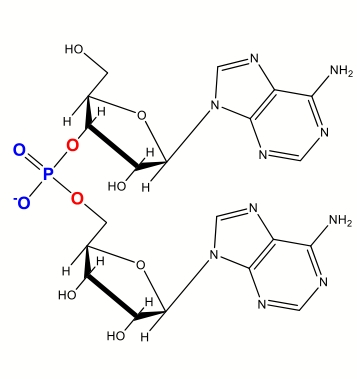
\includegraphics[width=\textwidth]{PhosphoDiesterBond}
	\end{subfigure}
	\begin{subfigure}[b]{0.45\textwidth}
		\centering
		\caption{Repels negatively charged nucleophiles which might break bond, so very stable}\label{fig:PhosphoDiesterBond1} 
		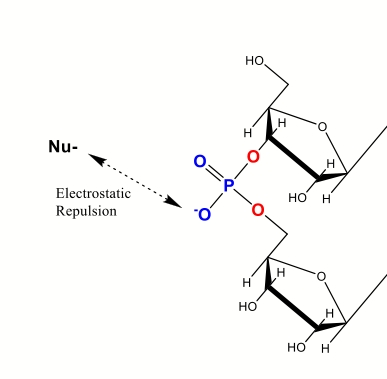
\includegraphics[width=\textwidth]{PhosphoDiesterBond1}
	\end{subfigure}
	\begin{subfigure}[b]{0.45\textwidth}
		\centering
		\caption{Bond is tunable if we need to react}\label{fig:PhosphoDiesterBond2} 
		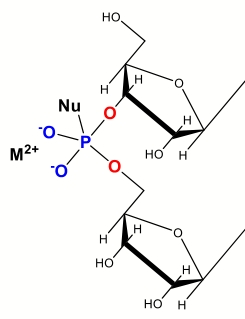
\includegraphics[width=\textwidth]{PhosphoDiesterBond2}
	\end{subfigure}
	\begin{subfigure}[b]{0.45\textwidth}
		\centering
		\caption{Repulsion keeps  soluble and prevents collapse}\label{fig:PhosphoDiesterBond3} 
		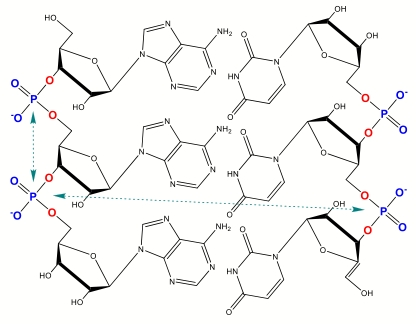
\includegraphics[width=\textwidth]{PhosphoDiesterBond3}
	\end{subfigure}
	
\end{figure}
\begin{figure}[H]
	\caption{Phospholipids}\label{fig:PhosphoLipids}
	
	\begin{subfigure}[b]{0.45\textwidth}
		\centering
		\caption{Phospho Diester Bond}\label{fig:PhosphoLipid1} 
		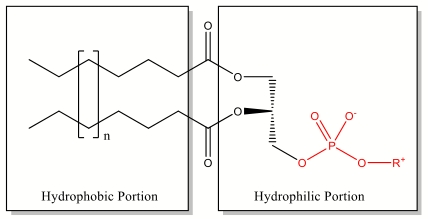
\includegraphics[width=\textwidth]{PhosphoLipid1}
	\end{subfigure}
	\begin{subfigure}[b]{0.45\textwidth}
		\centering
		\caption{Repels negatively charged nucleophiles which might break bond, so very stable}\label{fig:PhosphoLipid2} 
		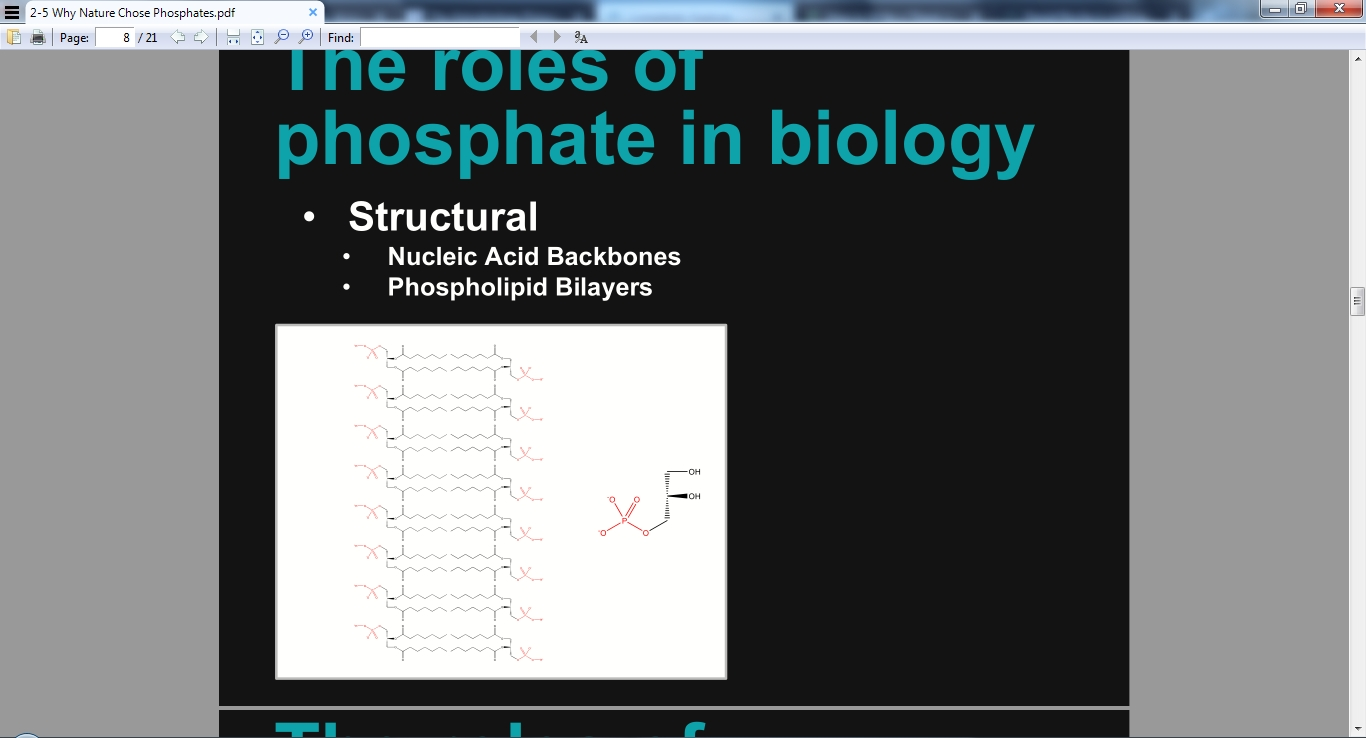
\includegraphics[width=\textwidth]{PhosphoLipid2}
	\end{subfigure}
	
	\begin{subfigure}[b]{0.45\textwidth}
		\centering
		\caption{Repulsion keeps \gls{gls:DNA} soluble and prevents collapse}\label{fig:PhosphoLipid3} 
		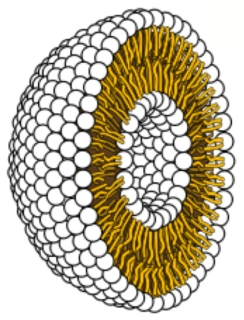
\includegraphics[width=\textwidth]{PhosphoLipid3}
	\end{subfigure}
	
\end{figure}

Why wouldn't you use phosphate?

\begin{itemize}
	\item Scarce
	\item Insoluble, unreactive
	\item No polyphosphate minerals
	\item One pyrophosphate mineral
	\item Limited geochemical production of reactive forms
\end{itemize}
Open Questions

\begin{itemize}
	\item When did life begin to use 	phosphate?
	\item If not at the very beginning, what 	came before?
	\item Where did early phosphate come 	from?
\end{itemize}

\section{Why Water? Why Carbon?}
Figures \ref{fig:abundances1} and \ref{fig:abundances2} show abundances. Figure \ref{fig:minerals} shows elements likely to be locked up in minerals, Figure \ref{fig:volatiles} shows elements that are likely to be in atmosphere or sea. Bonds are important - carbon has 4.

\begin{figure}[H]
	\caption{Abundance of Elements in the Solar System}\label{fig:abundances1} 
	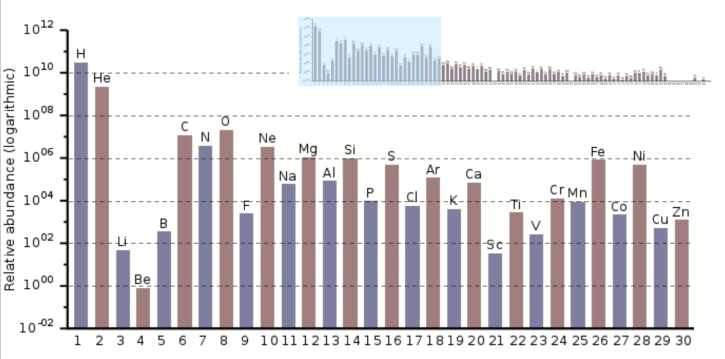
\includegraphics[width=0.9\textwidth]{Abundances}
\end{figure}

\begin{figure}[H]
	\caption{Abundance of Elements in the Earth's Crust}\label{fig:abundances2}  
	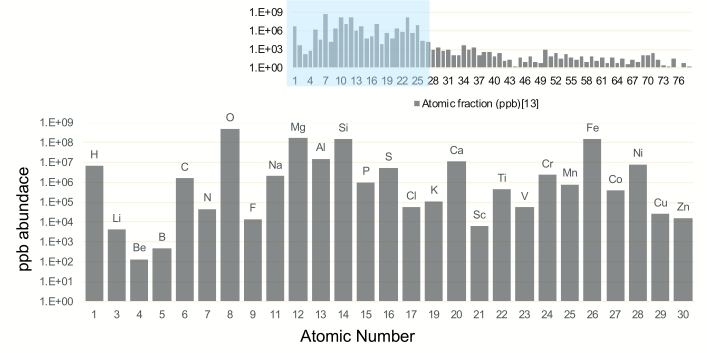
\includegraphics[width=0.9\textwidth]{AbundancesEarth}
\end{figure}

\begin{figure}[H]
	\caption{Some elements locked in minerals}\label{fig:minerals} 
	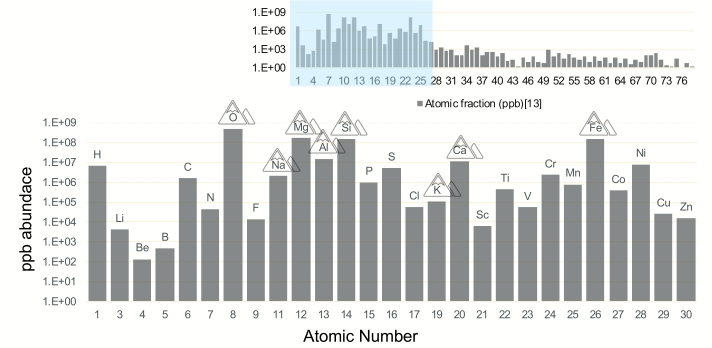
\includegraphics[width=0.9\textwidth]{AbundancesMinerals}
\end{figure}

\begin{figure}[H]
	\caption{Some elements volatile}\label{fig:volatiles} 
	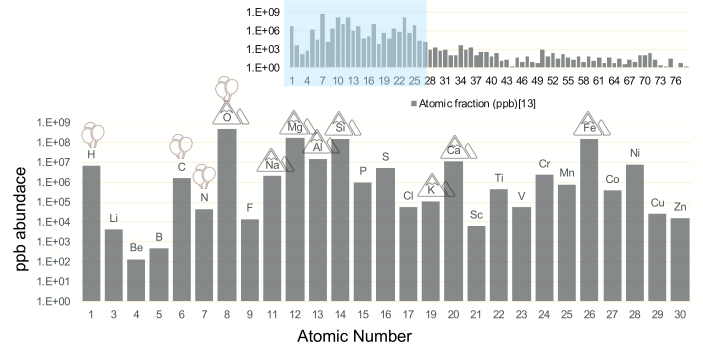
\includegraphics[width=0.9\textwidth]{AbundancesGases}
\end{figure}

Water is abundant, stable, and a liquid.

What are the other possibilities?
\begin{itemize}
	\item Silicon
	\begin{itemize}
		\item Can adopt similar structures to carbon
		\item Poor reactivity with many other elements
		\item Reactive with water
	\end{itemize}
	\item Borane
	\begin{itemize}
		\item Diverse Chemistry
		\item Unstable in Oxidizing Environment
		\item Low Cosmic Abundance
	\end{itemize}
	\item Metal Oxides (?)
\begin{itemize}
	\item 	Less diverse chemistry
	\item Demonstrated biomimetic functions
\end{itemize}
\end{itemize}

What are the other possibilities for solvents?
\begin{itemize}
	\item Ammonia
	\item Urea
	\item Formamide
	\item Alkanes
\end{itemize}

Open Questions
\begin{itemize}
	\item What are the surface and atmospheric chemistries of
	exoplanets?
	\item How much of extant biochemistry can be accomplished
	in other solvents?
	\item How much of extant biochemistry can be mimicked with
	other substrates?
\end{itemize}
\section{Macromolecules}

Sarah Maurer

\subsection{Proteins}

\cite[25.9 Proteins]{brown2009chemistry}

\begin{figure}[H]
	\caption{The full set of 20 amino acids: blue atoms form protein backbone. There are a couple of extra amino acids used for some organisms.}\label{fig:AminoAcids} 
	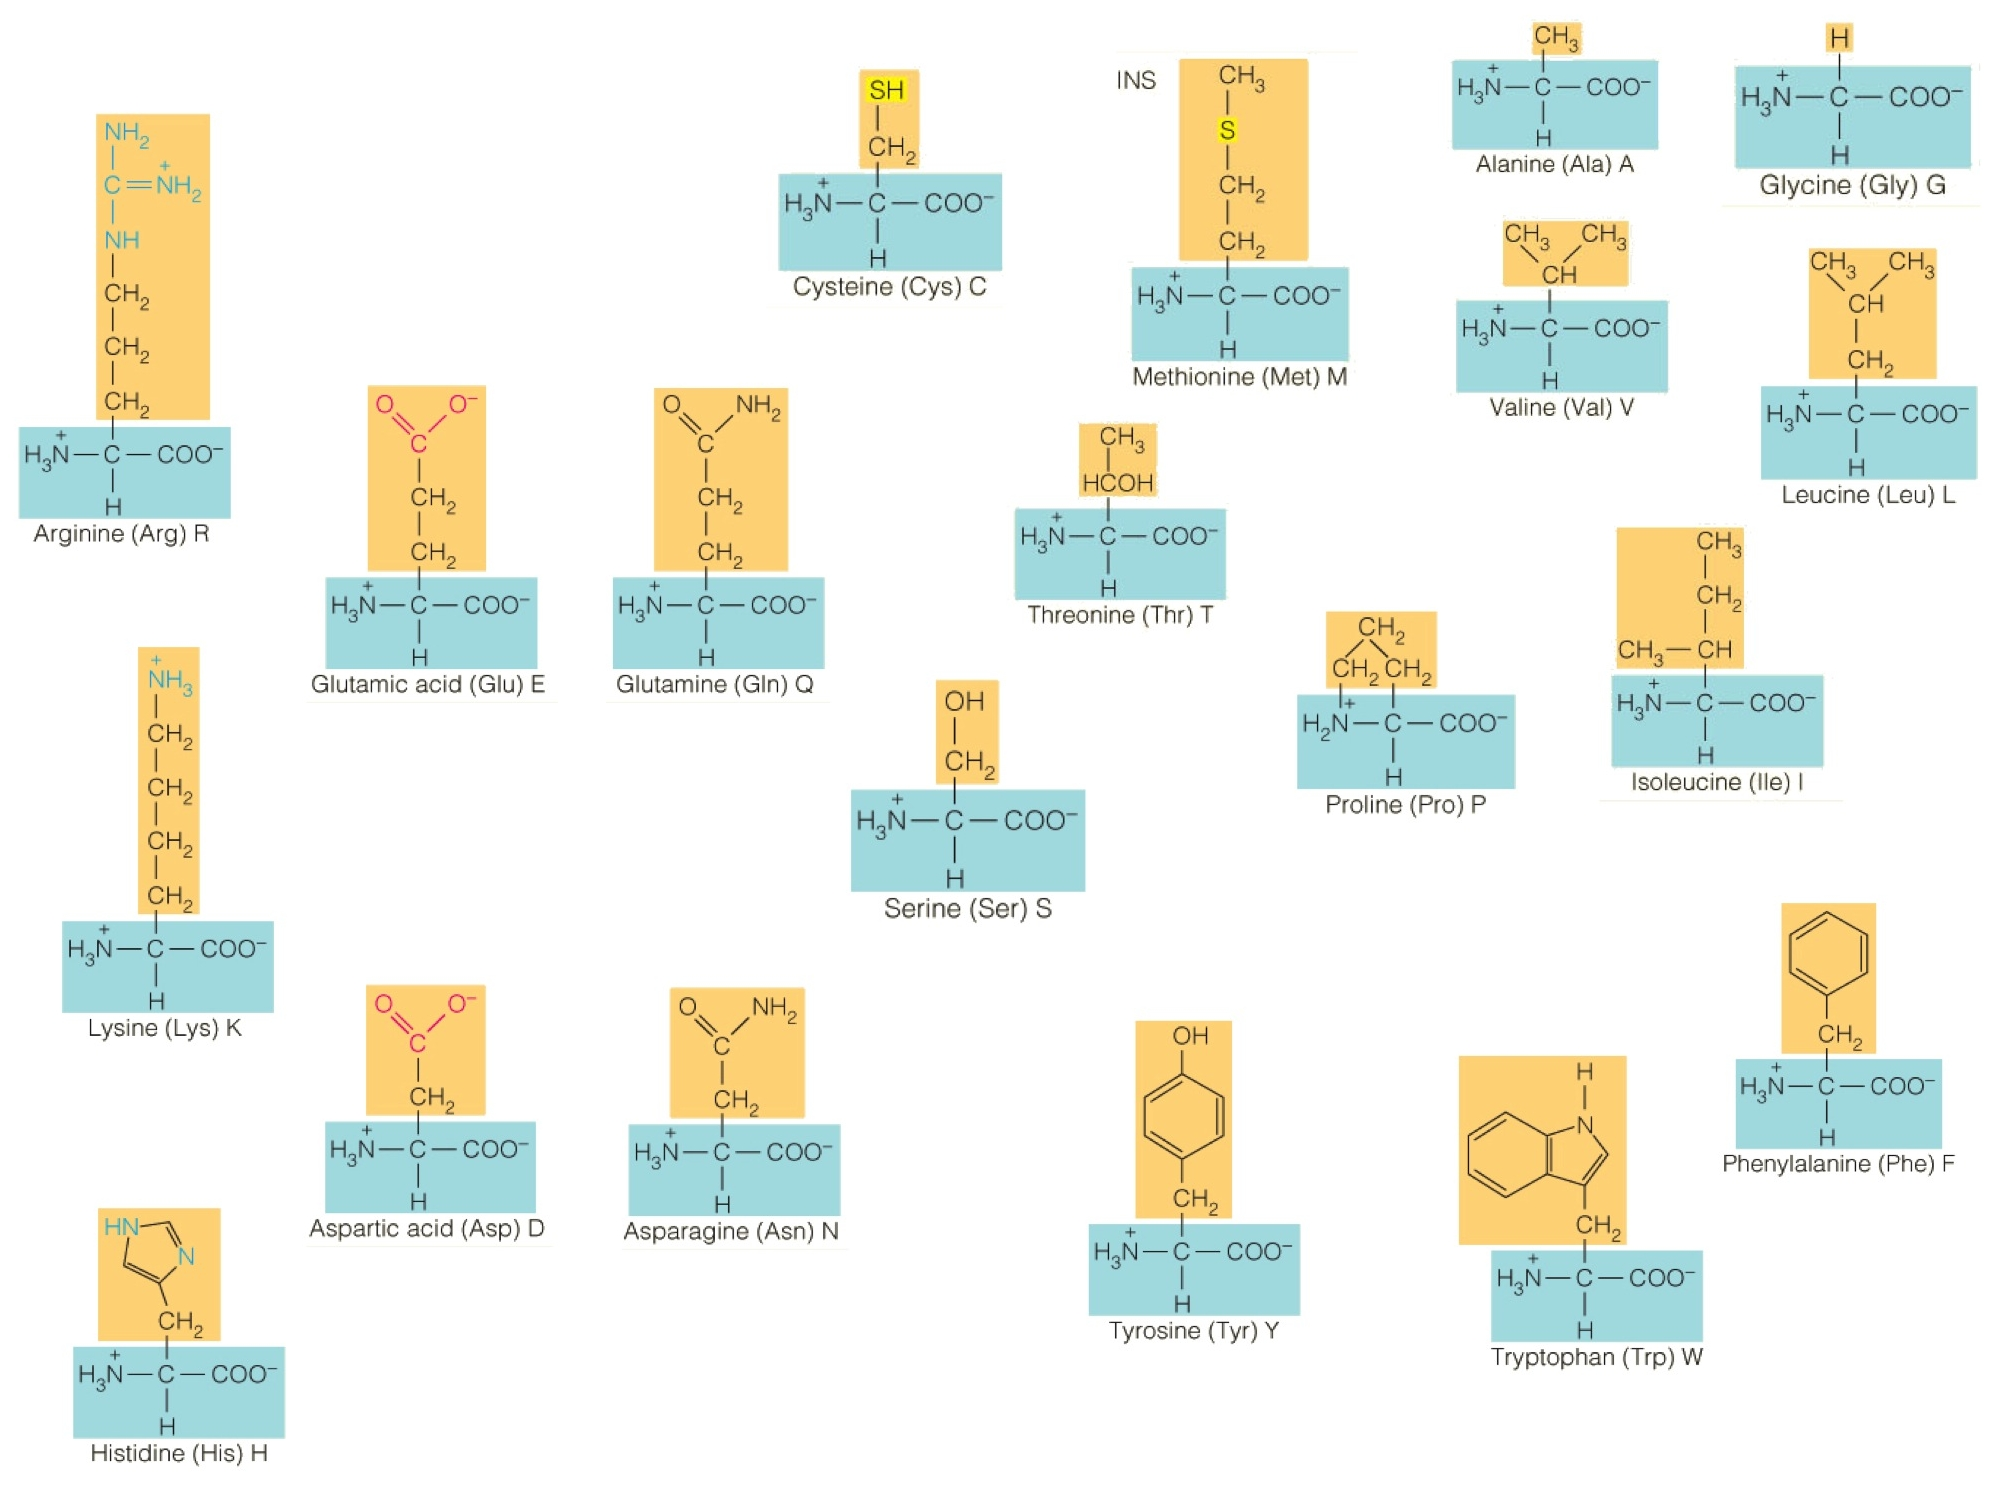
\includegraphics[width=0.9\textwidth]{AminoAcids}
\end{figure}

\begin{figure}[H]
	\caption{Amino acids grouped by charge.}\label{fig:AminoAcidsGrouped} 
	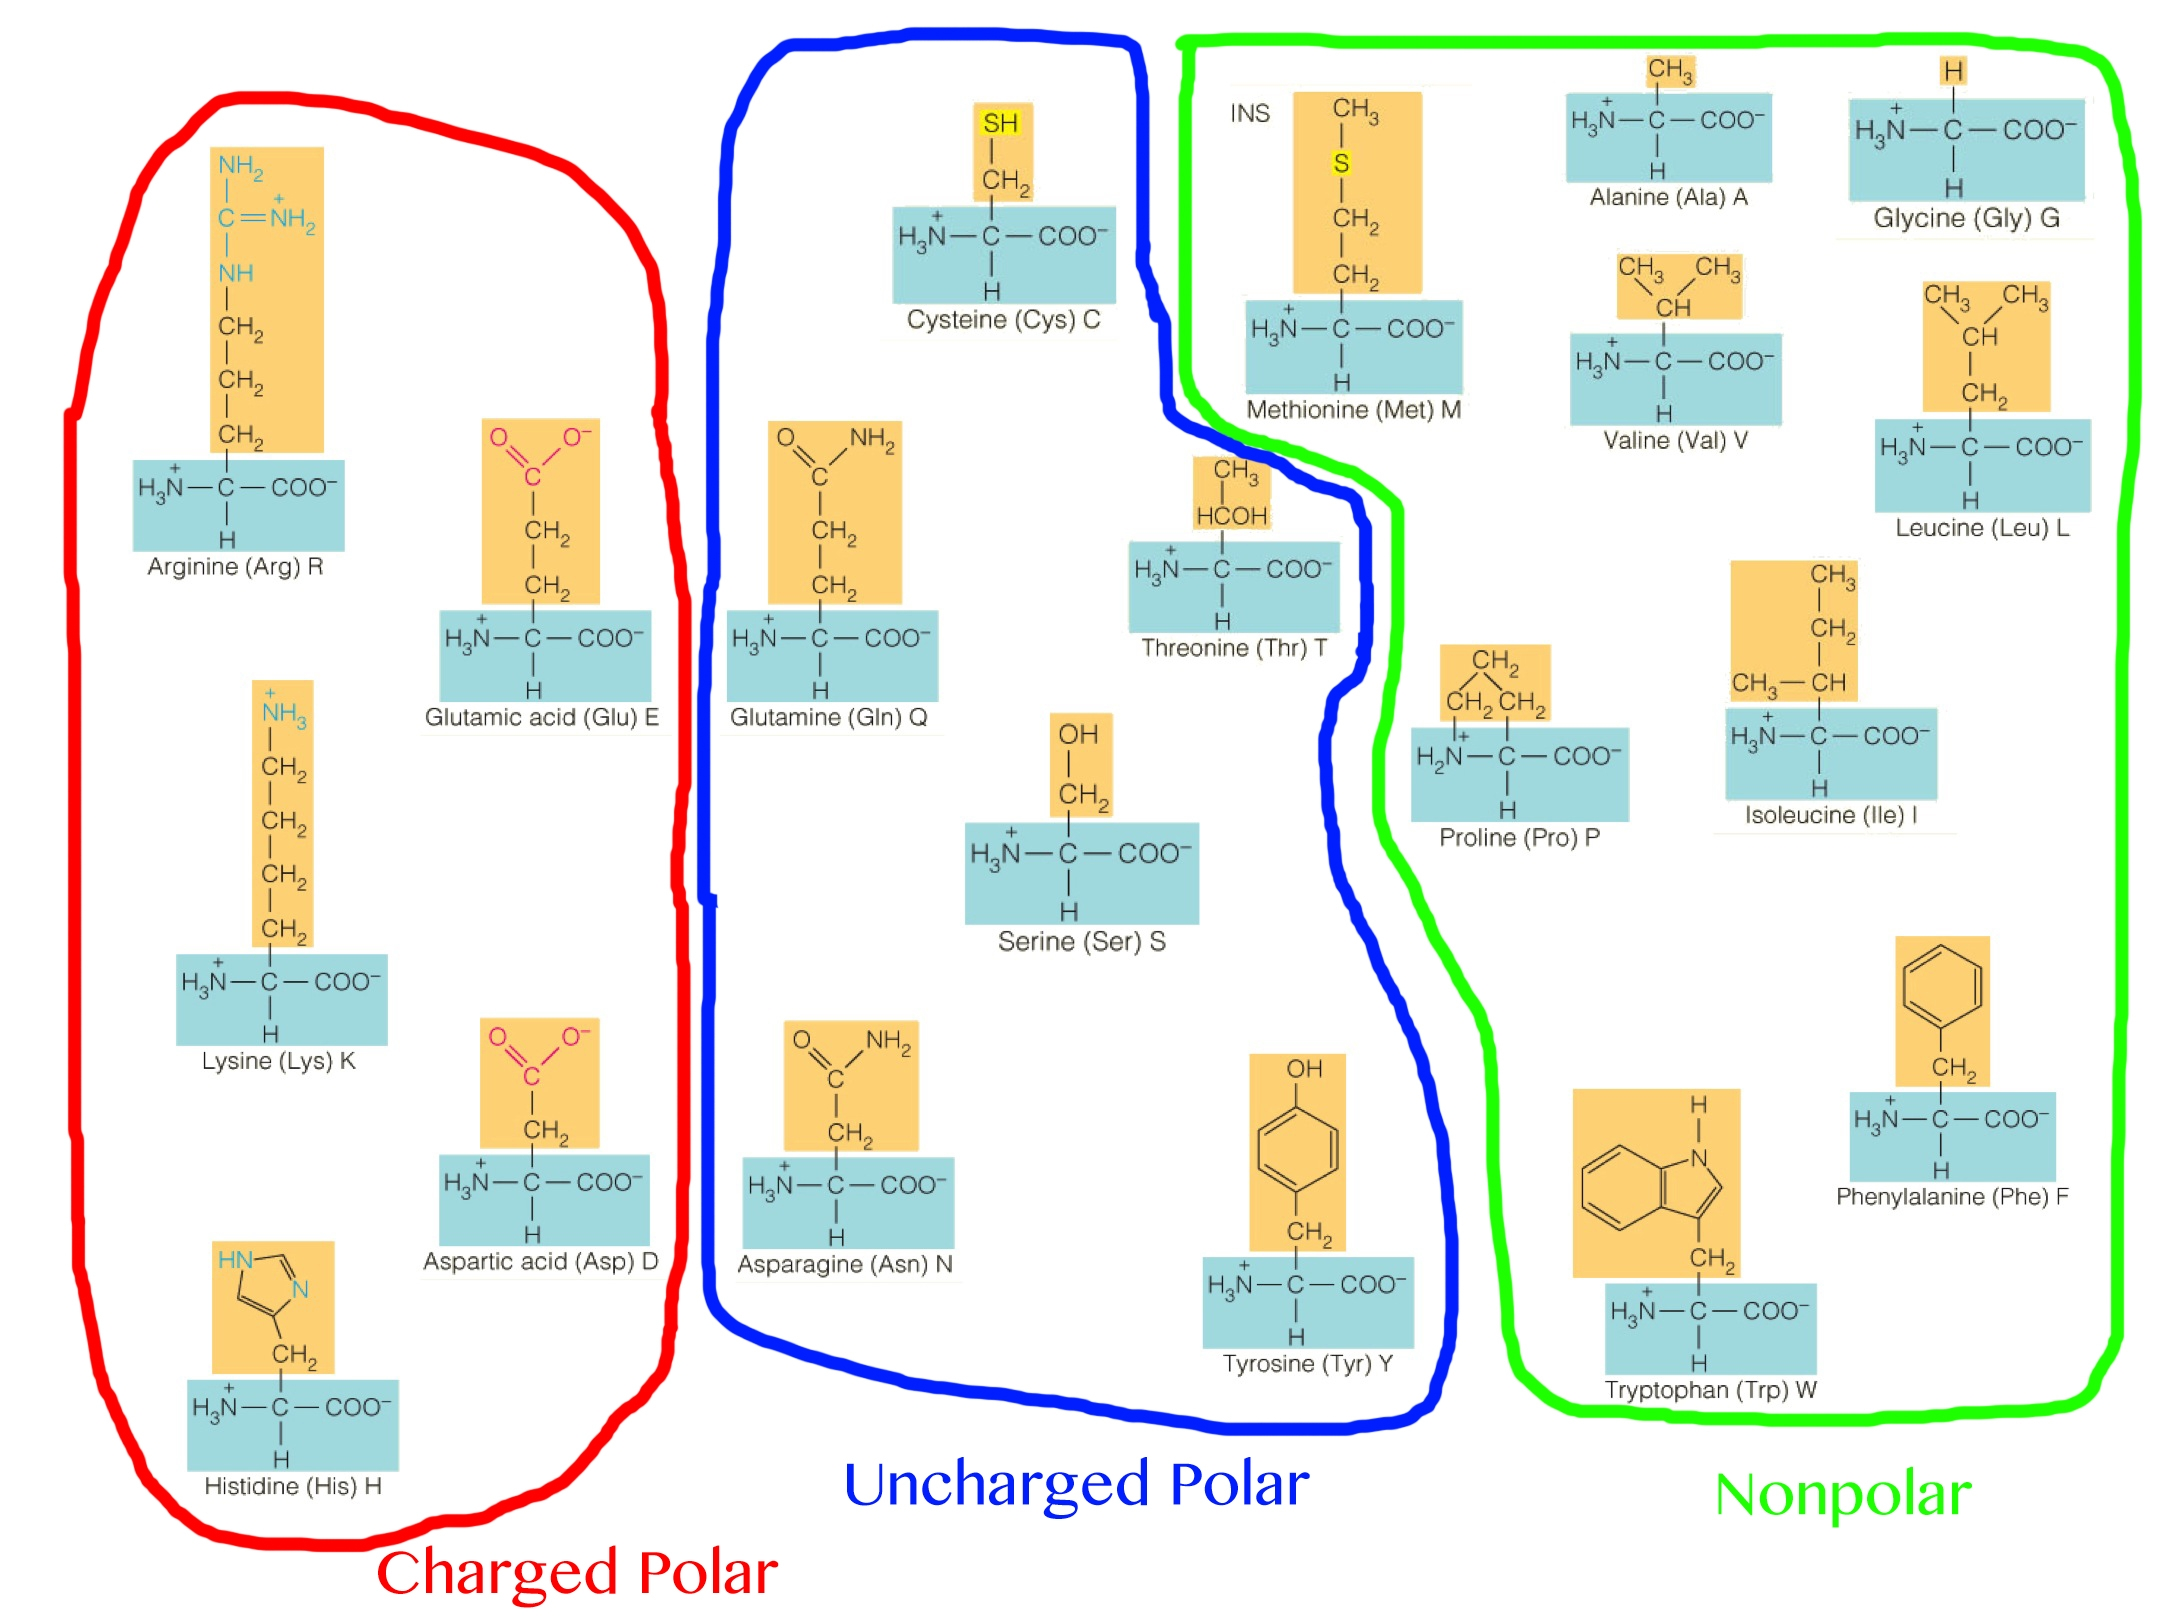
\includegraphics[width=0.9\textwidth]{AminoAcidsGrouped}
\end{figure}

\begin{figure}[H]
	\caption{Condensing amino acids by removing $H_2O$. Dehydration.}\label{fig:AminoAcidsCondensed} 
	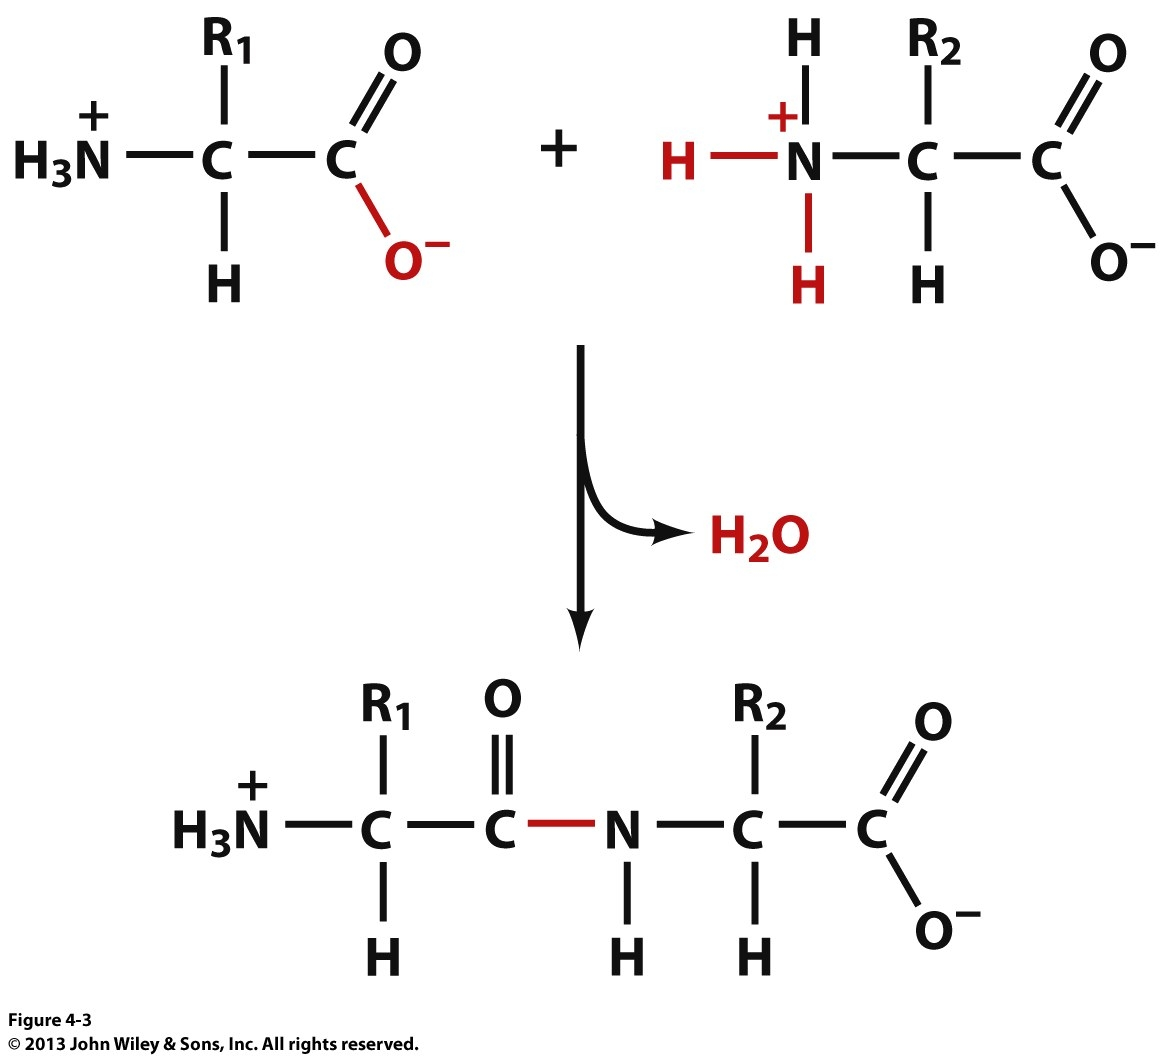
\includegraphics[width=0.9\textwidth]{AminoAcidsCondensed}
\end{figure}

\begin{itemize}
	\item  Specifically target recognition (due to folded
	structure) - lock and key mechanism
	\item  Need at least several amino acids to have
	folded stability, most proteins are 50+ amino
	acids
	\item We would need protein formation to happen many times on early Earth.
	\item Enzymes are catalysts
	\begin{itemize}
		\item Lower transition state energy
		\item Orient and concentrate reactants, so they react more quickly than if floating around in solution.
	\end{itemize}
\end{itemize}



\subsection{Lipids}
\cite[14.2 Lipids \& Triglycerides]{brown2009chemistry}

\begin{itemize}
	\item Phospholipids make up modern cell
	membranes
	\item amphiphilic molecules can also form
	membranes
\end{itemize}

\begin{figure}[H]
	\caption{Lipids form hydrophobic membranes that surround cells, and allow Darwinian evolution.}\label{fig:Lipids} 
	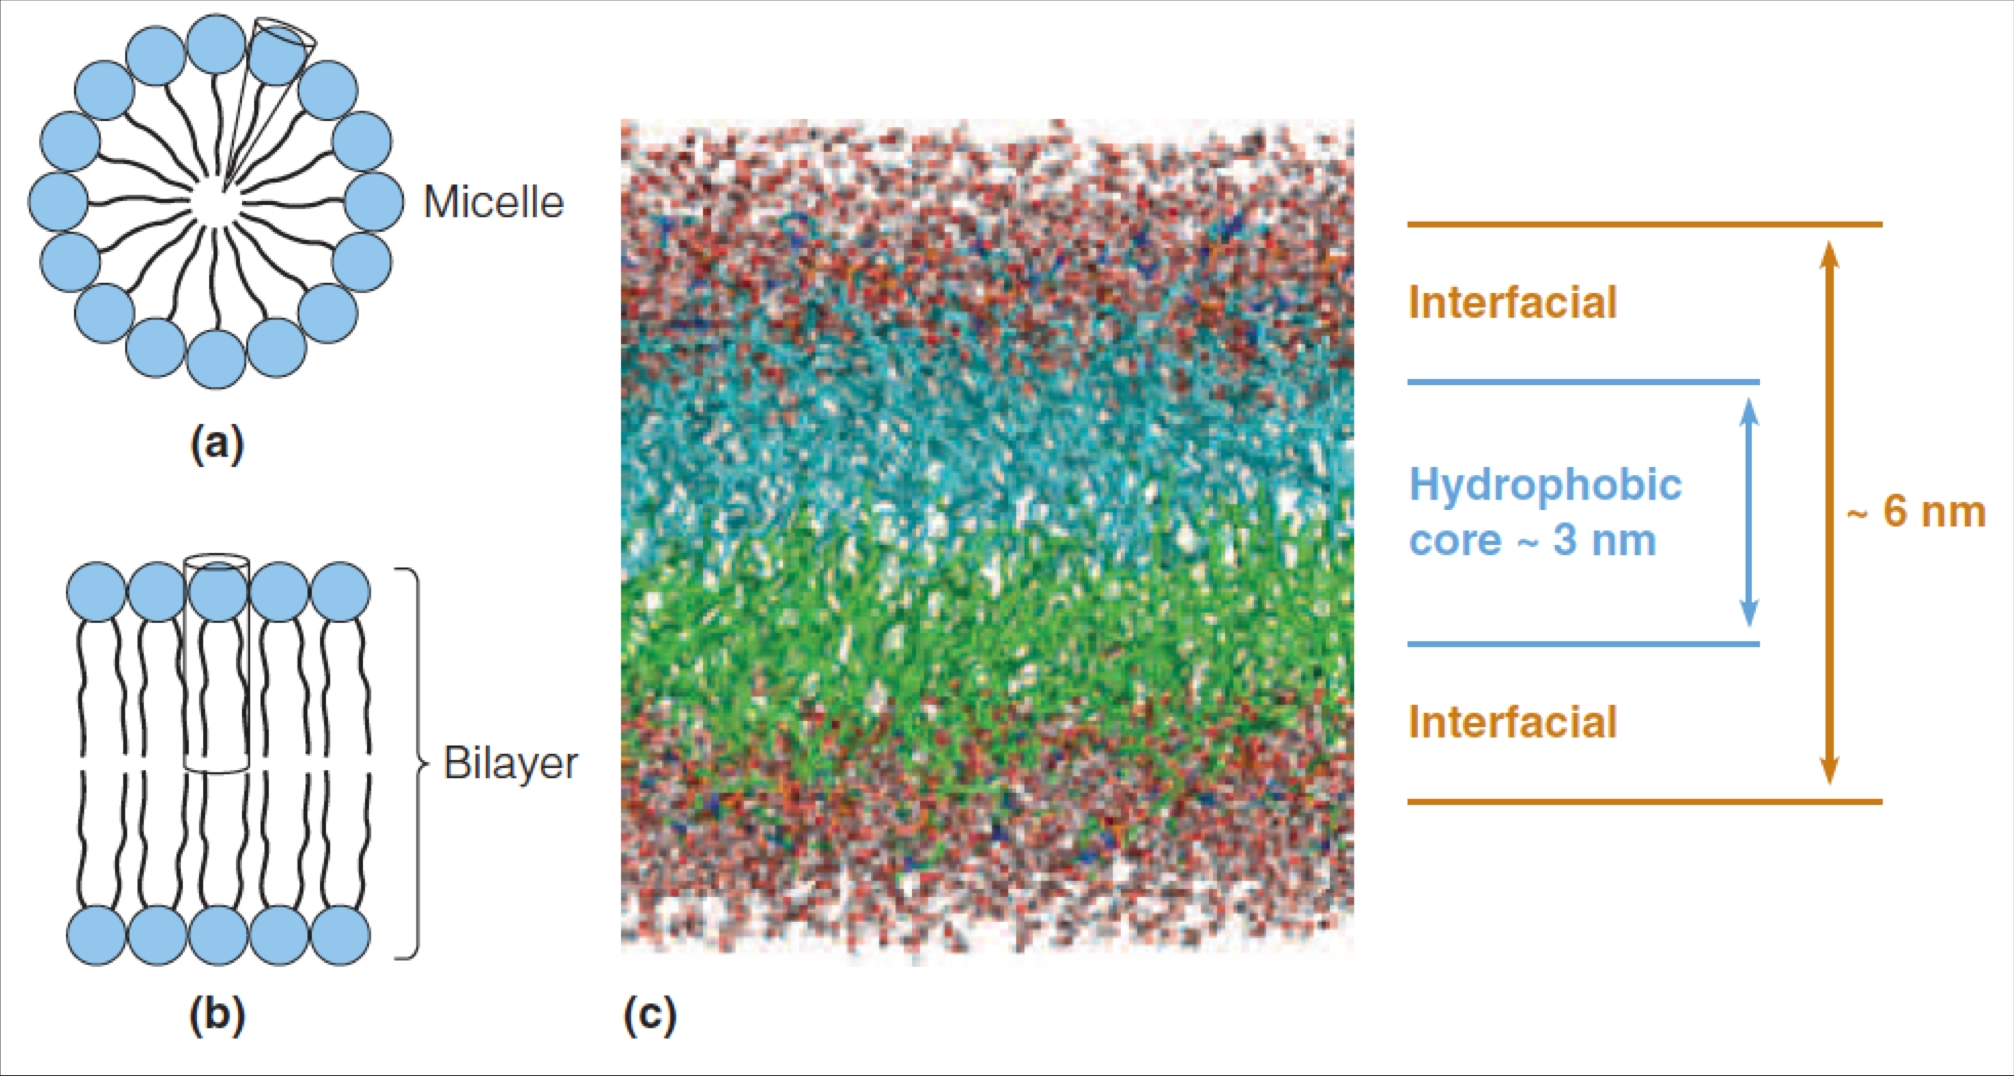
\includegraphics[width=0.9\textwidth]{Lipids}
\end{figure}

\begin{figure}[H]
	\caption{Type of lipid depends on head-group (blue). NB, some membranes, in Achaea, are monolayer, not bilayer.}\label{fig:LipidTypes} 
	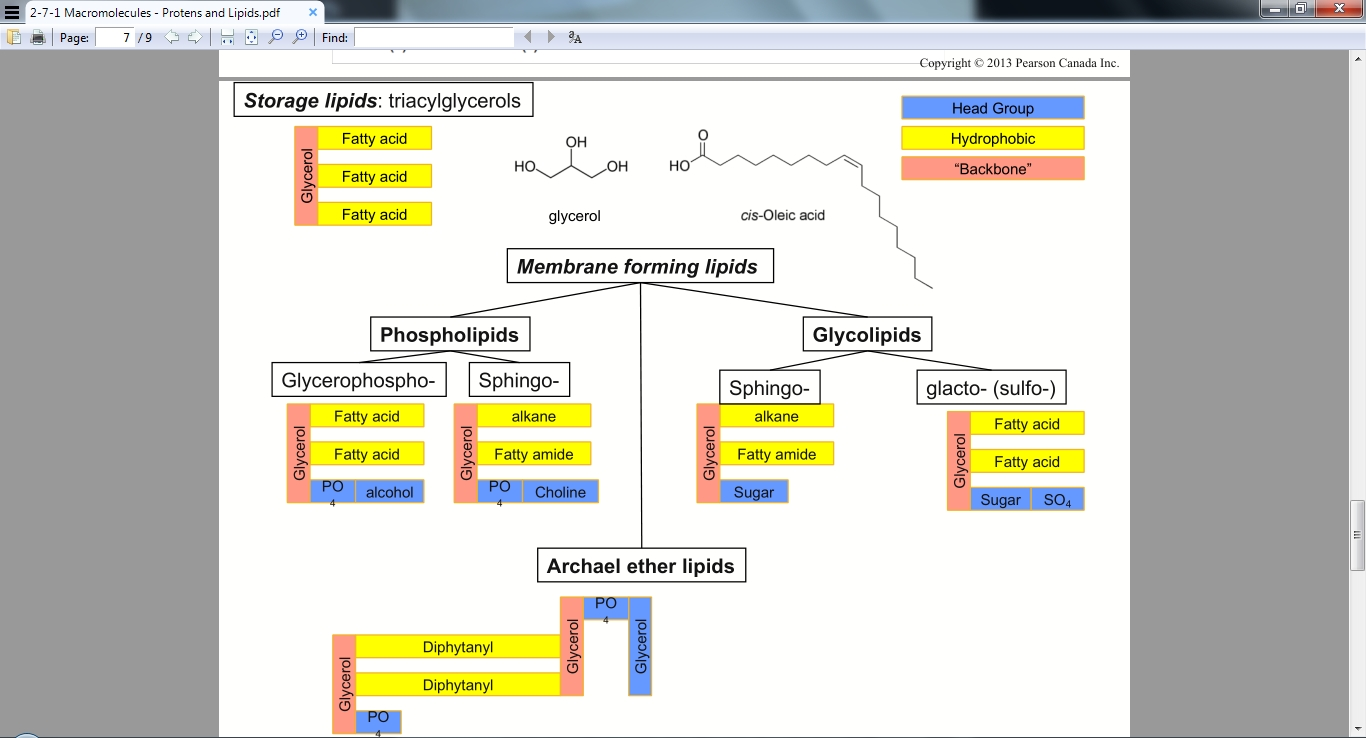
\includegraphics[width=0.9\textwidth]{LipidTypes}
\end{figure}

\begin{itemize}
	\item Single chain amphiphiles with with chemically
	diverse headgroups
	\item Less stable than phospholipids
	\item Figure \ref{fig:SimplerLipids} sows some example. Left one has been found in meteorites.
\end{itemize}
\begin{figure}[H]
	\caption{Early life would have used simple lipids.}\label{fig:SimplerLipids} 
	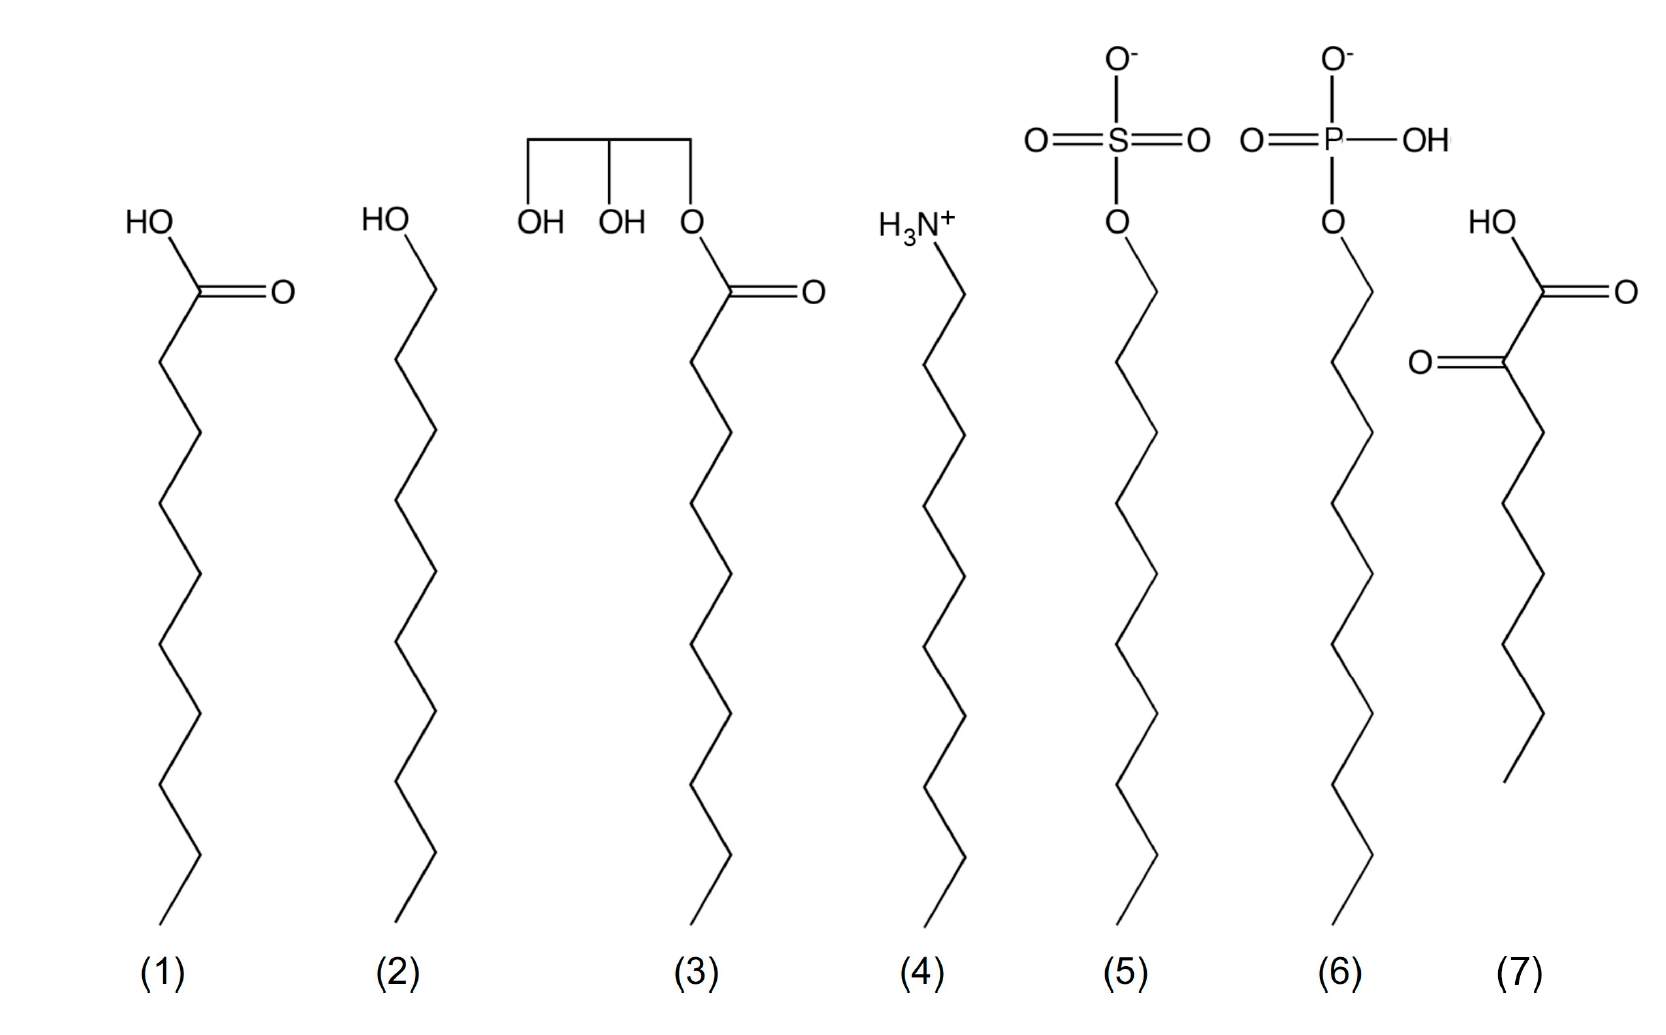
\includegraphics[width=0.9\textwidth]{SimplerLipids}
\end{figure}

\subsection{Sugars}
\begin{itemize}
	\item Role in biological systems:
	\item generating and storing biological energy
	\item molecular recognition (as in the immune system)
	\item cellular protection (as in bacterial and plant cell 	walls)
	\item maintaining biological structure (e.g., cellulose).
	\item controlling protein trafficking
	\item cell signaling
	\item cell adhesion
	\item biological lubricants
\end{itemize}

\begin{figure}[H]
	\caption{Sugars: generating and storing biological energy.}\label{fig:SugarsCycle} 
	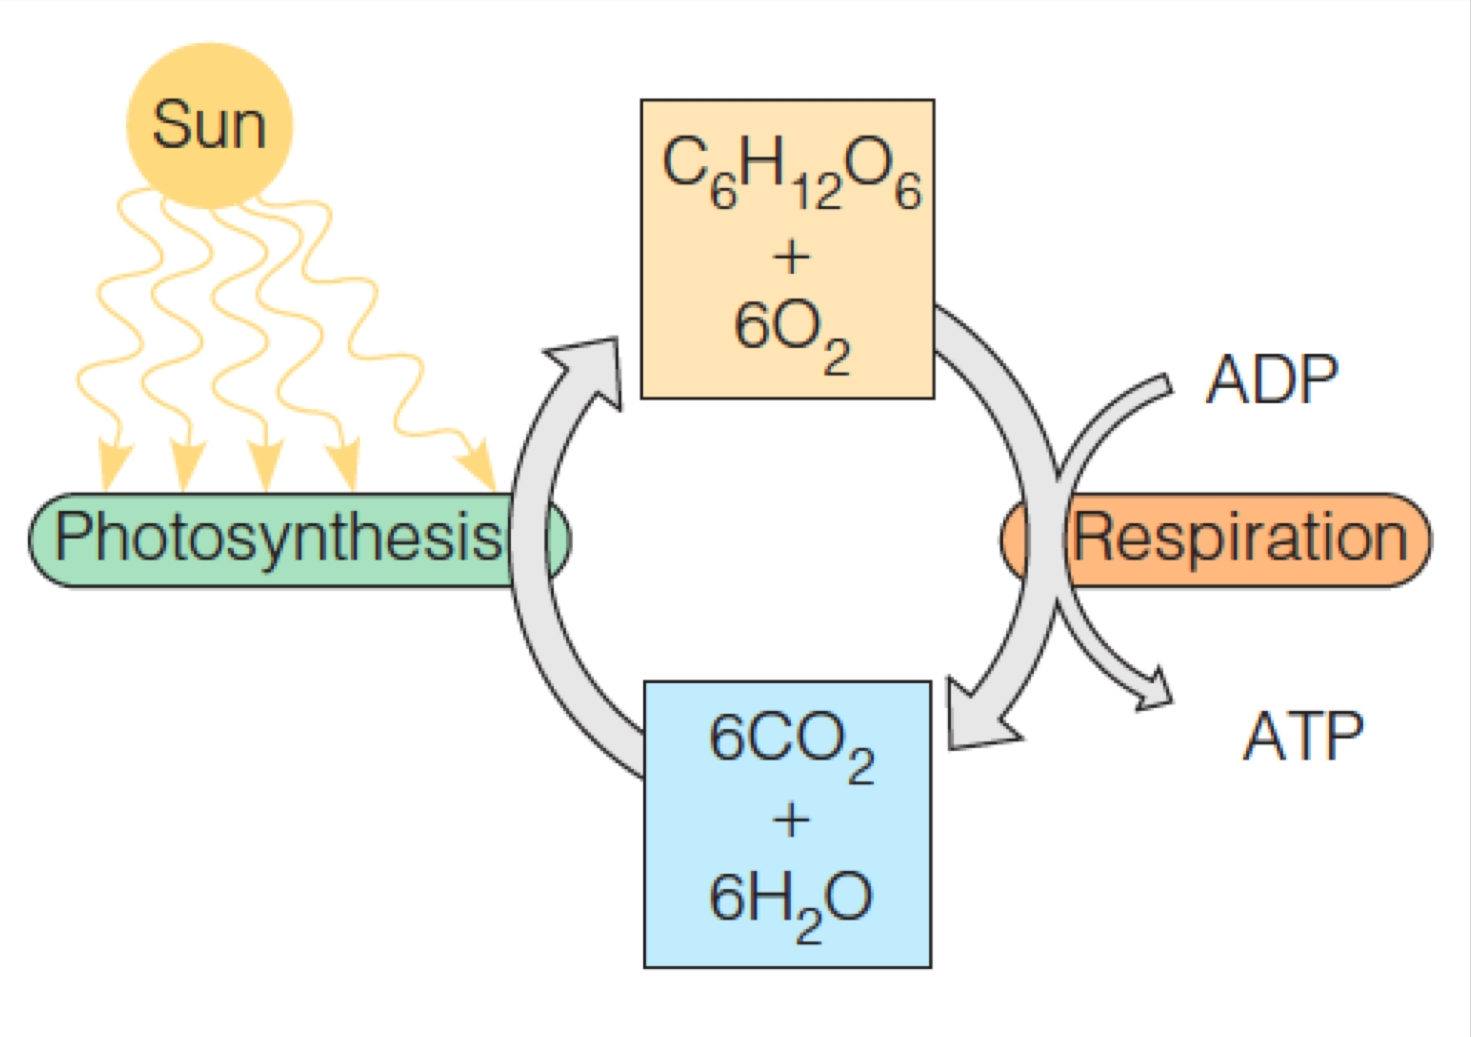
\includegraphics[width=0.9\textwidth]{SugarsCycle}
\end{figure}

\begin{figure}[H]
	\caption{Variety of D-\glspl{gls:aldose}}\label{fig:SugarsStructure} 
	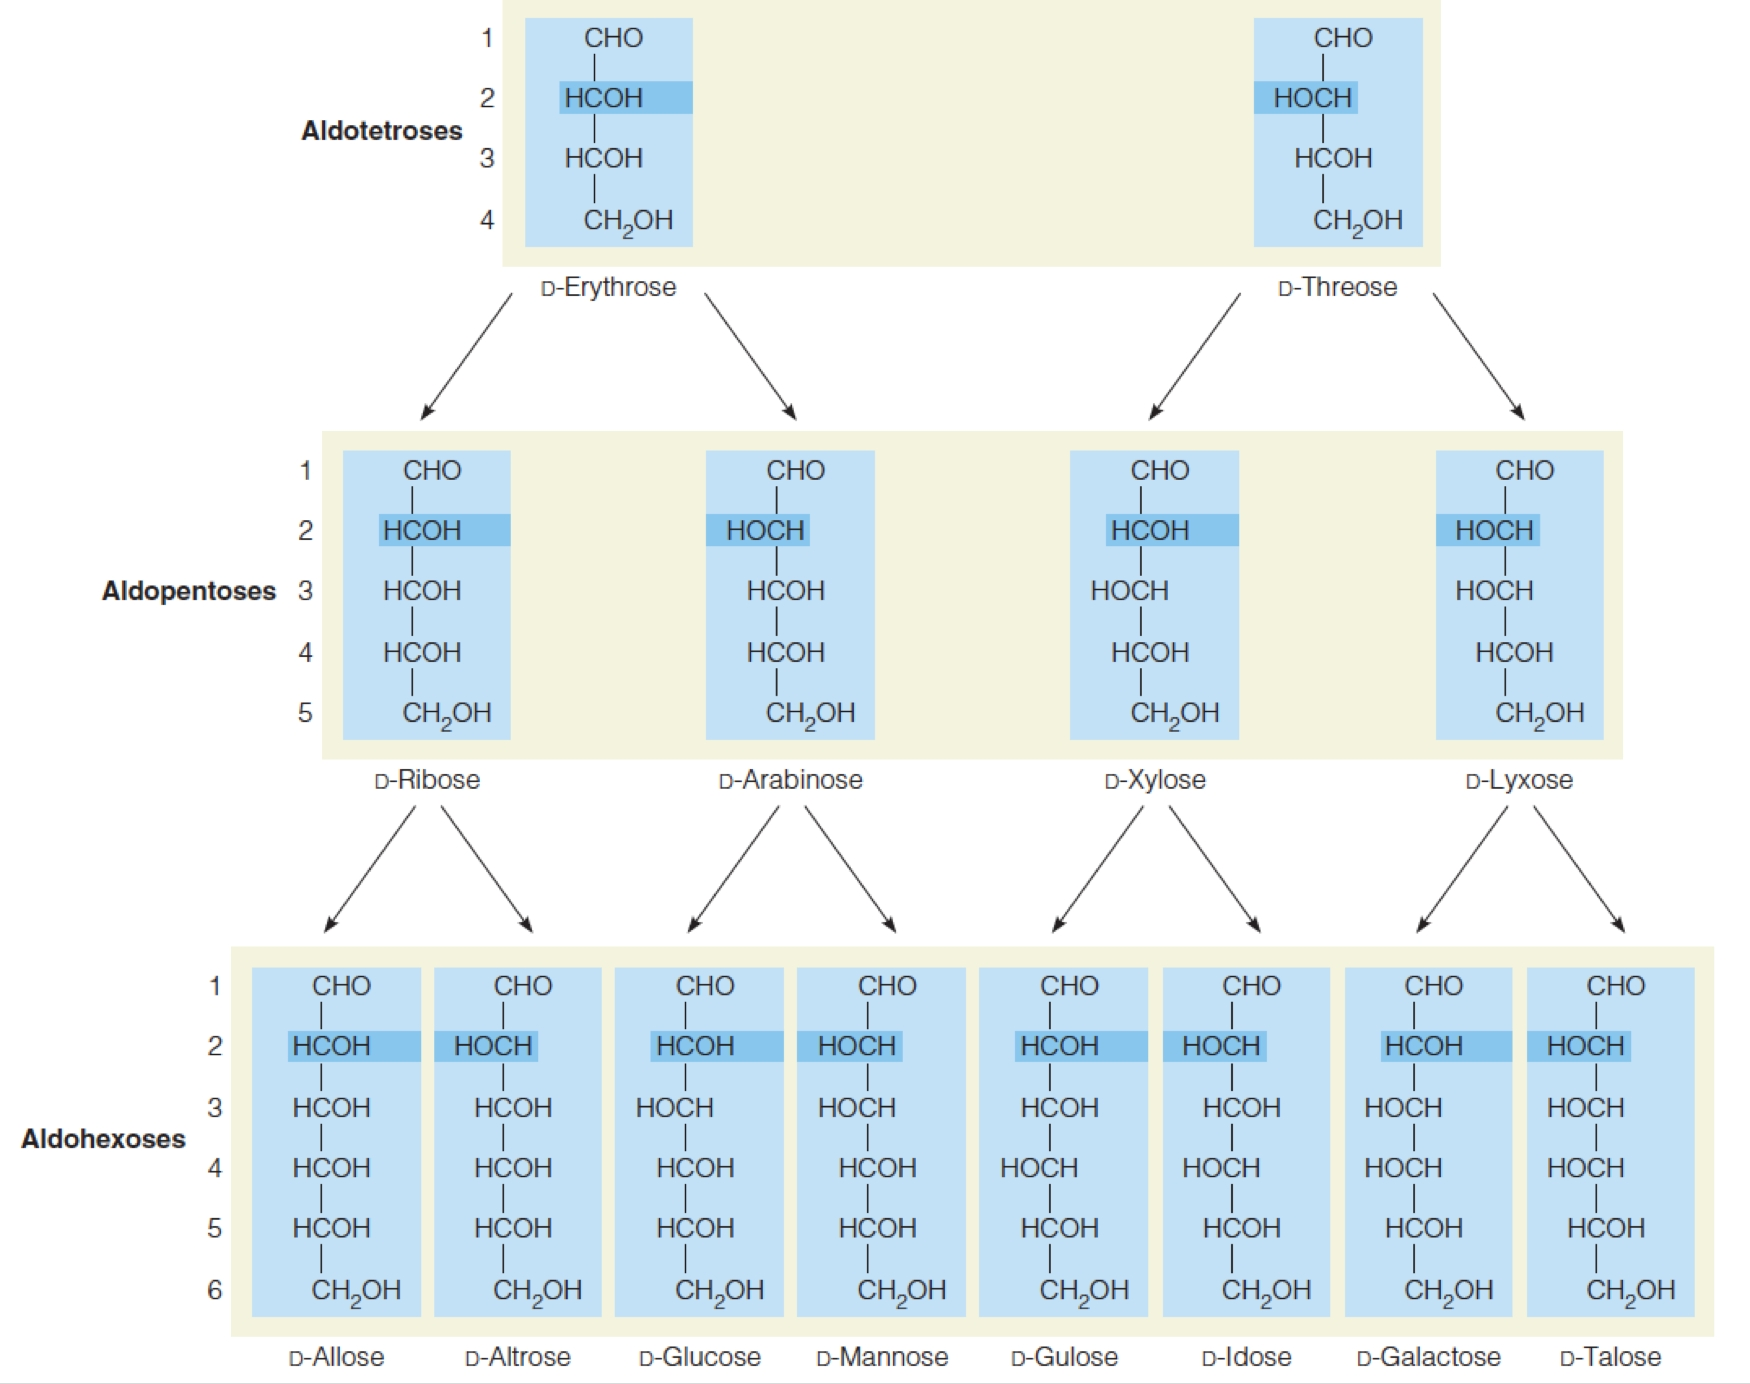
\includegraphics[width=0.9\textwidth]{SugarsStructure}
\end{figure}

\begin{figure}[H]
	\caption{Variety of D-ketoses}\label{fig:ketoses} 
	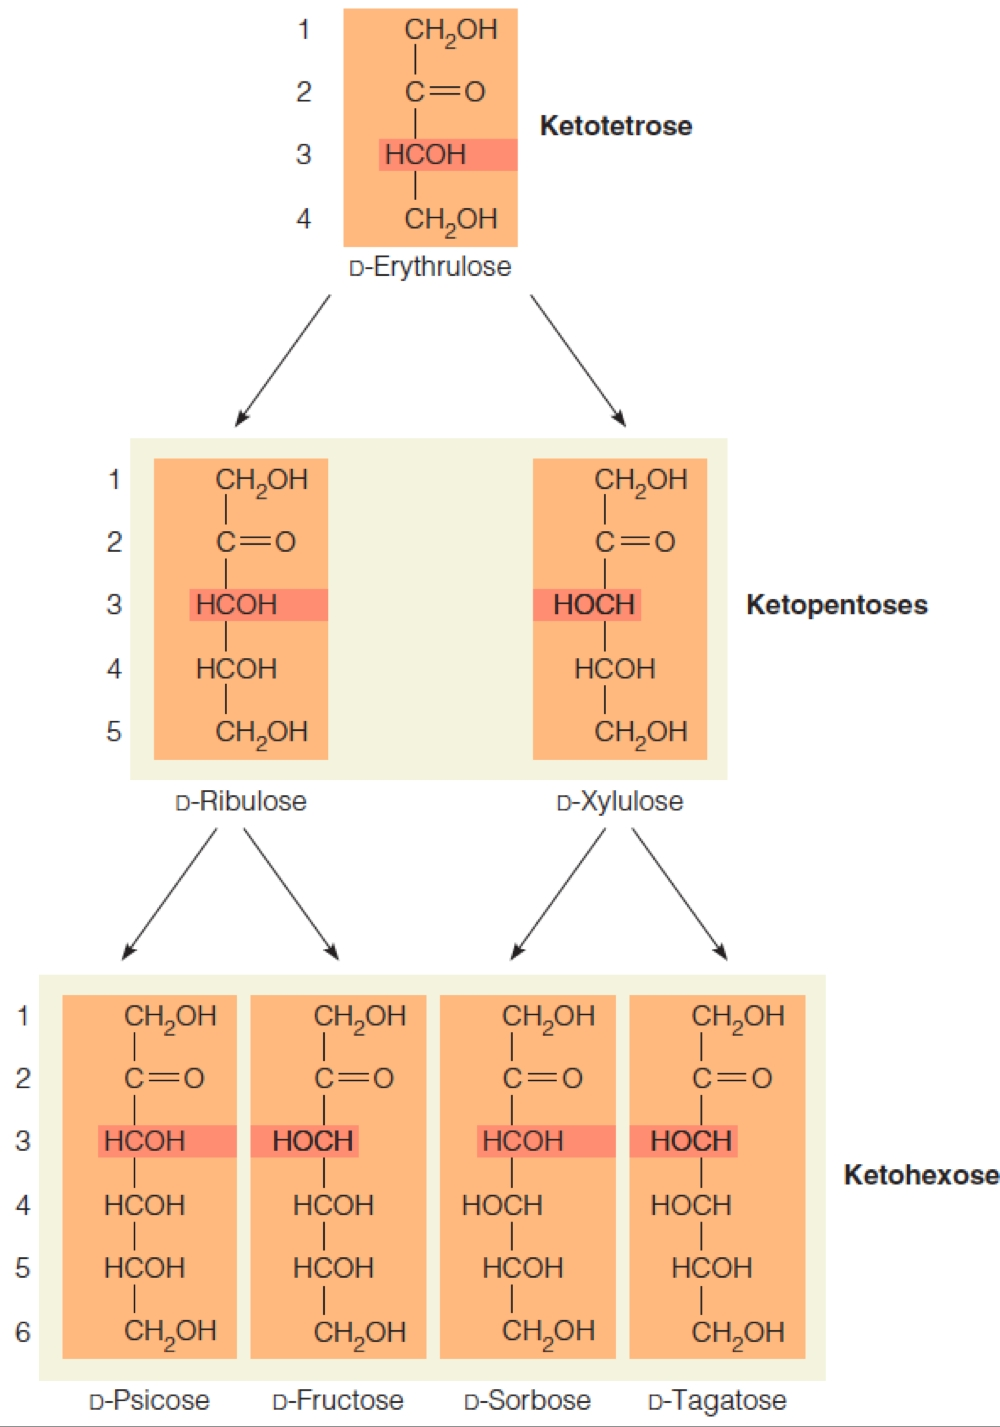
\includegraphics[width=0.9\textwidth]{ketoses}
\end{figure}


\begin{itemize}
	\item Ribose is usually rolled up into \gls{gls:pyran} (6 member ring) or \gls{gls:furan}(5)
	\item Reactive OH group (green in Figure \ref{fig:SugarTautomers}), anomeric Oxygen, can be at bottom ($alpha$) or top($beta$). This is where polymerization happens. RNA uses $\beta-furanose$, so we need enzymes to make this type.
\end{itemize}
\begin{figure}[H]
	\caption{Sugars are usually not linear: can accomplish different functions, depending on shape.}\label{fig:SugarTautomers} 
	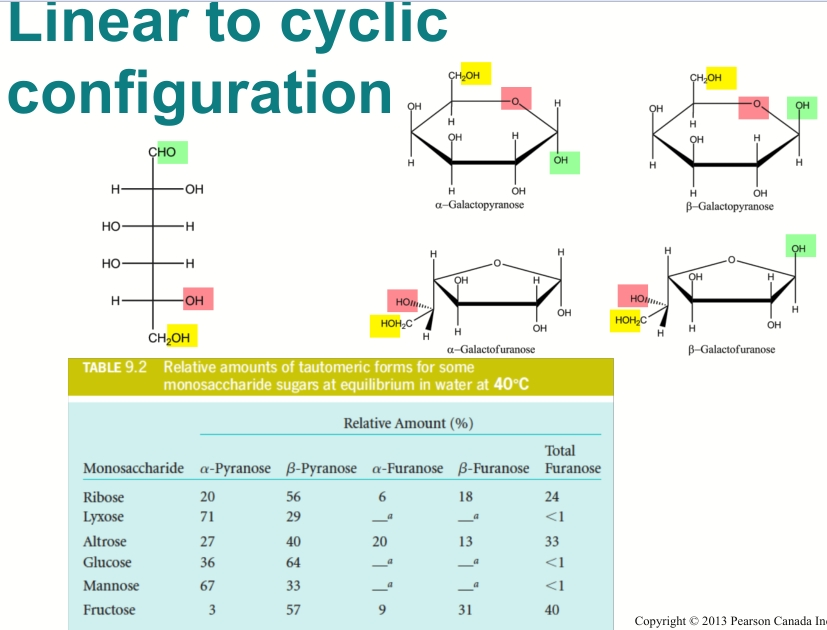
\includegraphics[width=0.9\textwidth]{SugarTautomers}
\end{figure}

\begin{figure}[H]
	\caption{Prebiotic synthesis of sugars: formose reaction. As the reaction progresses an insoluble “tar” forms an sugar concentrations decrease!}\label{fig:SugarsPrebioticSynthesis} 
	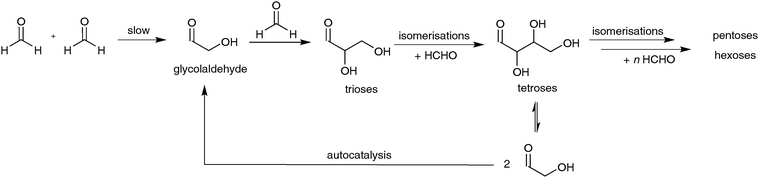
\includegraphics[width=0.9\textwidth]{SugarsPrebioticSynthesis}
\end{figure}

\subsection{Nucleic Acids}

\begin{figure}[H]
	\caption{The two types of heterocyclic bases are
		derivatives of purine and of pyrimidine.}\label{fig:Nucleobases} 
	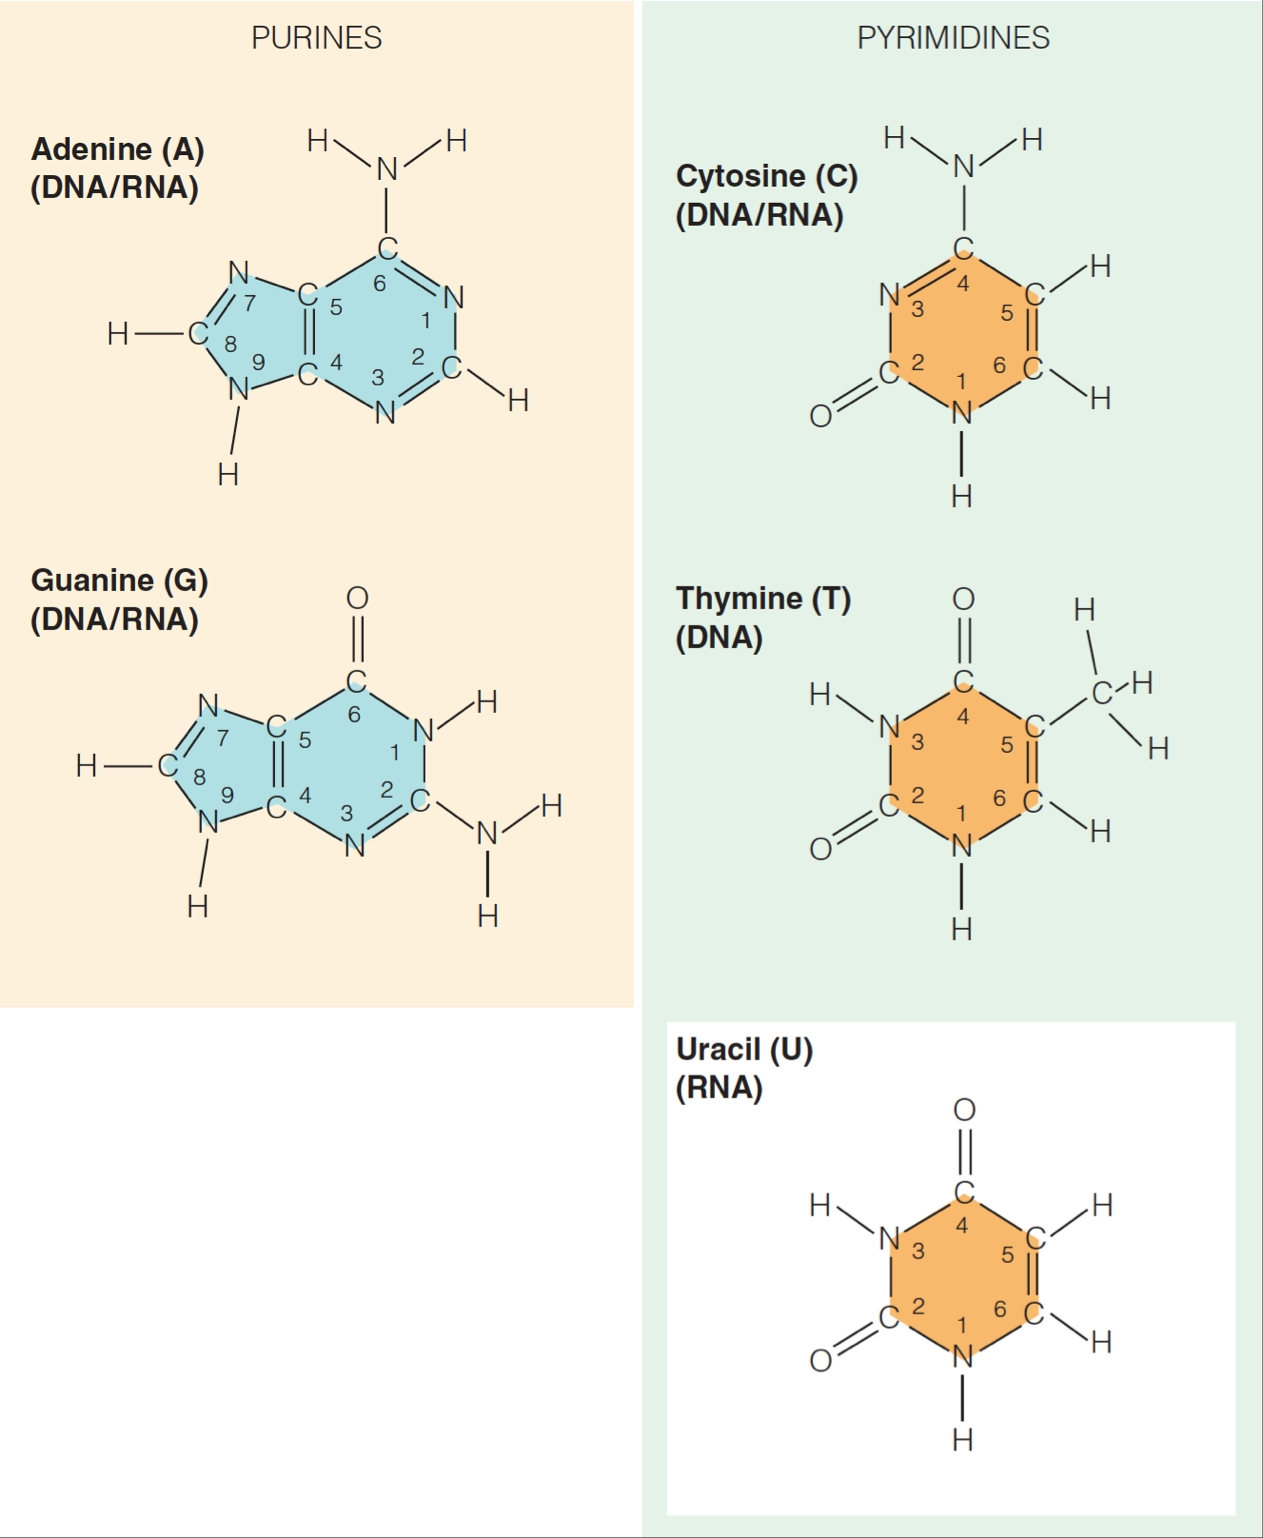
\includegraphics[width=0.9\textwidth]{Nucleobases}
\end{figure}

\begin{figure}[H]
	\caption{A-T (2 H-bonds) and G-C (3 H-bonds) are the base pairs in the Watson–
		Crick model of \gls{gls:DNA}.}\label{fig:BasePairs} 
	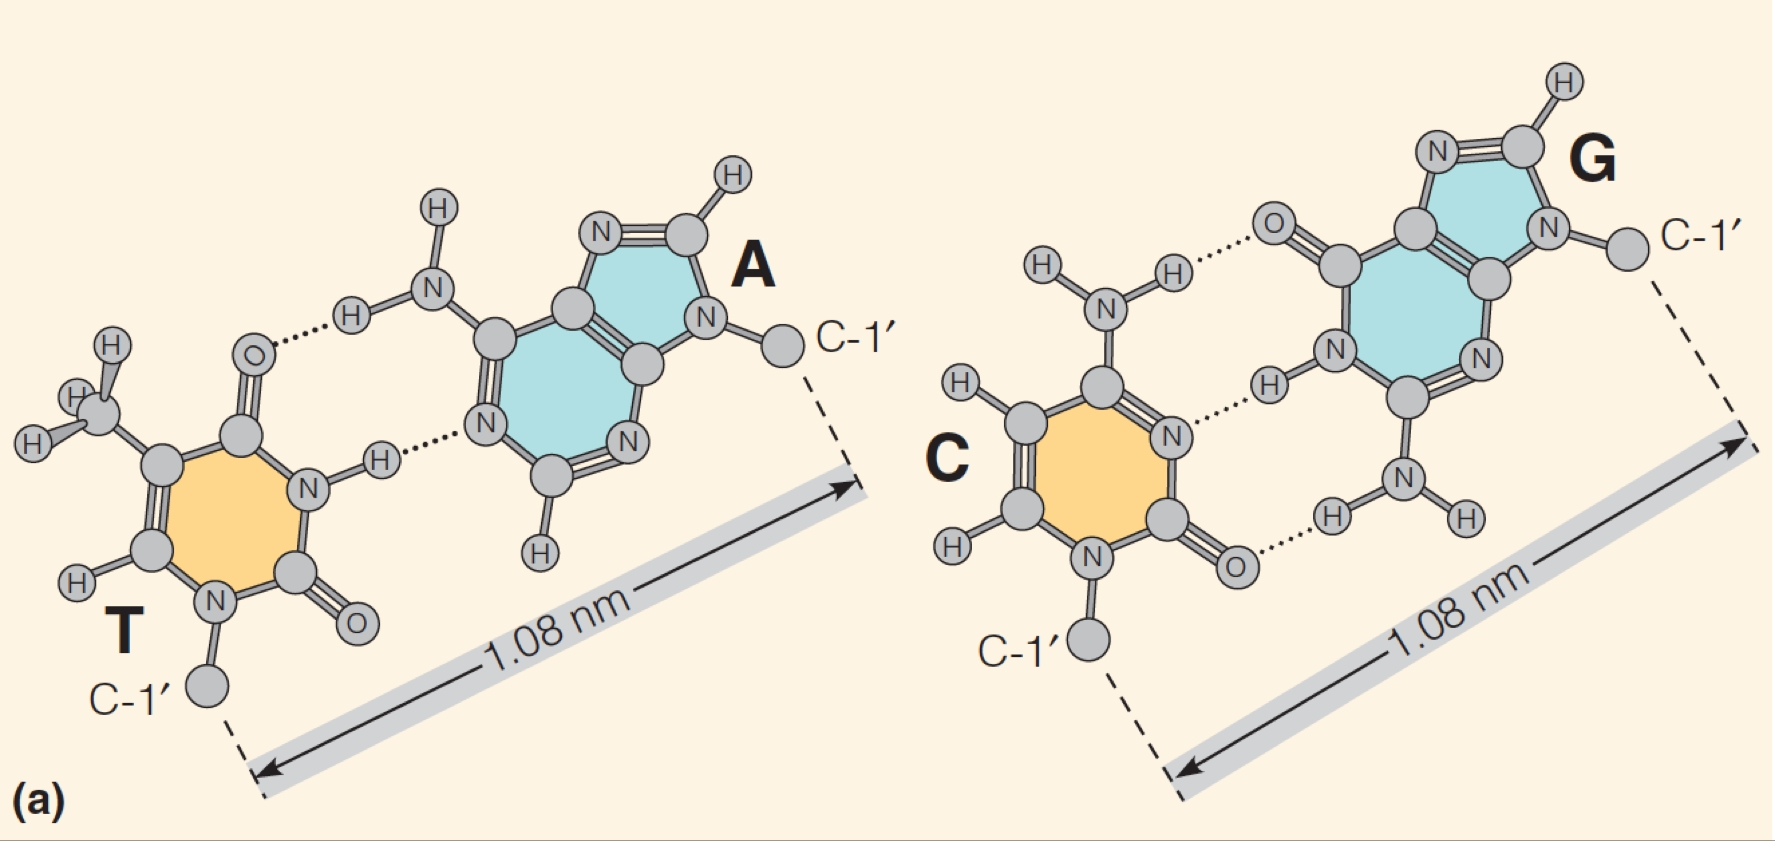
\includegraphics[width=0.9\textwidth]{BasePairs}
\end{figure}

\begin{figure}[H]
	\caption{Prebiotic synthesis is challenging, but not impossible!}\label{fig:PrebioticSynthesis} 
	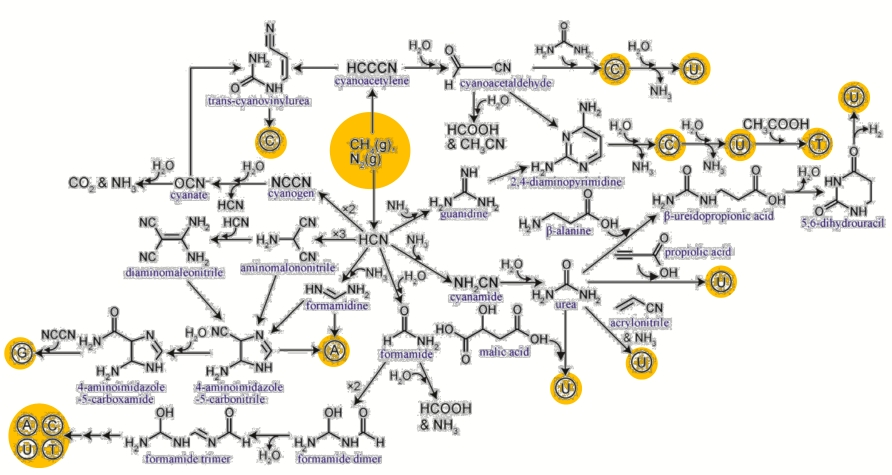
\includegraphics[width=0.9\textwidth]{PrebioticSynthesis}
\end{figure}

\begin{figure}[H]
	\caption{Nucleotide Structure. RNA loses OH group, so it can't hydrogen bind into complex structures the way \gls{gls:DNA} does. Ribose and phosphate make up backbone. Bases on outside, so can basepair.}\label{fig:NucleotideStructure} 
	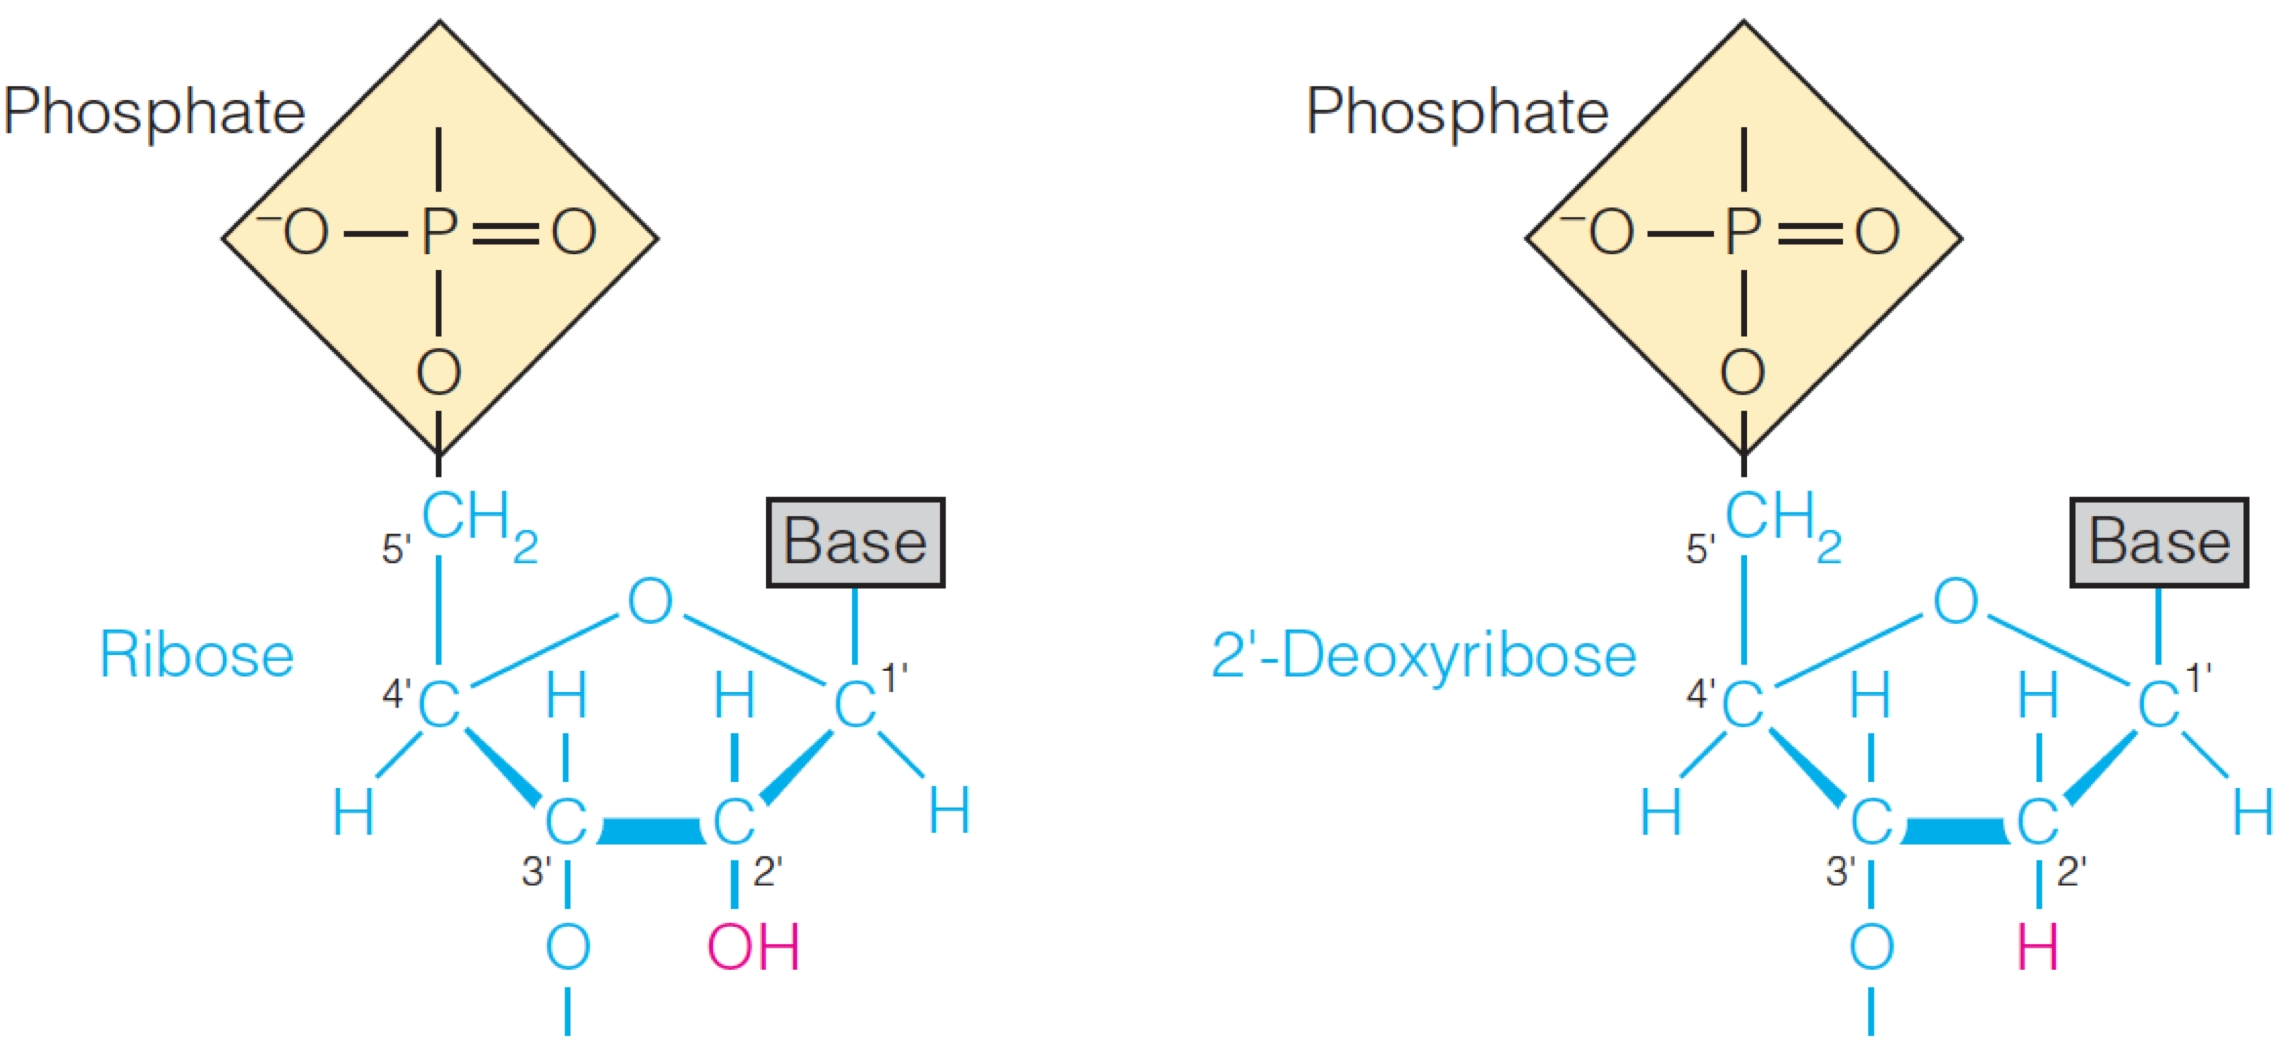
\includegraphics[width=0.9\textwidth]{NucleotideStructure}
\end{figure}

\begin{figure}[H]
	\caption{Nucleic Acid
		Polymers.}\label{fig:NucleicAcidPolymers} 
	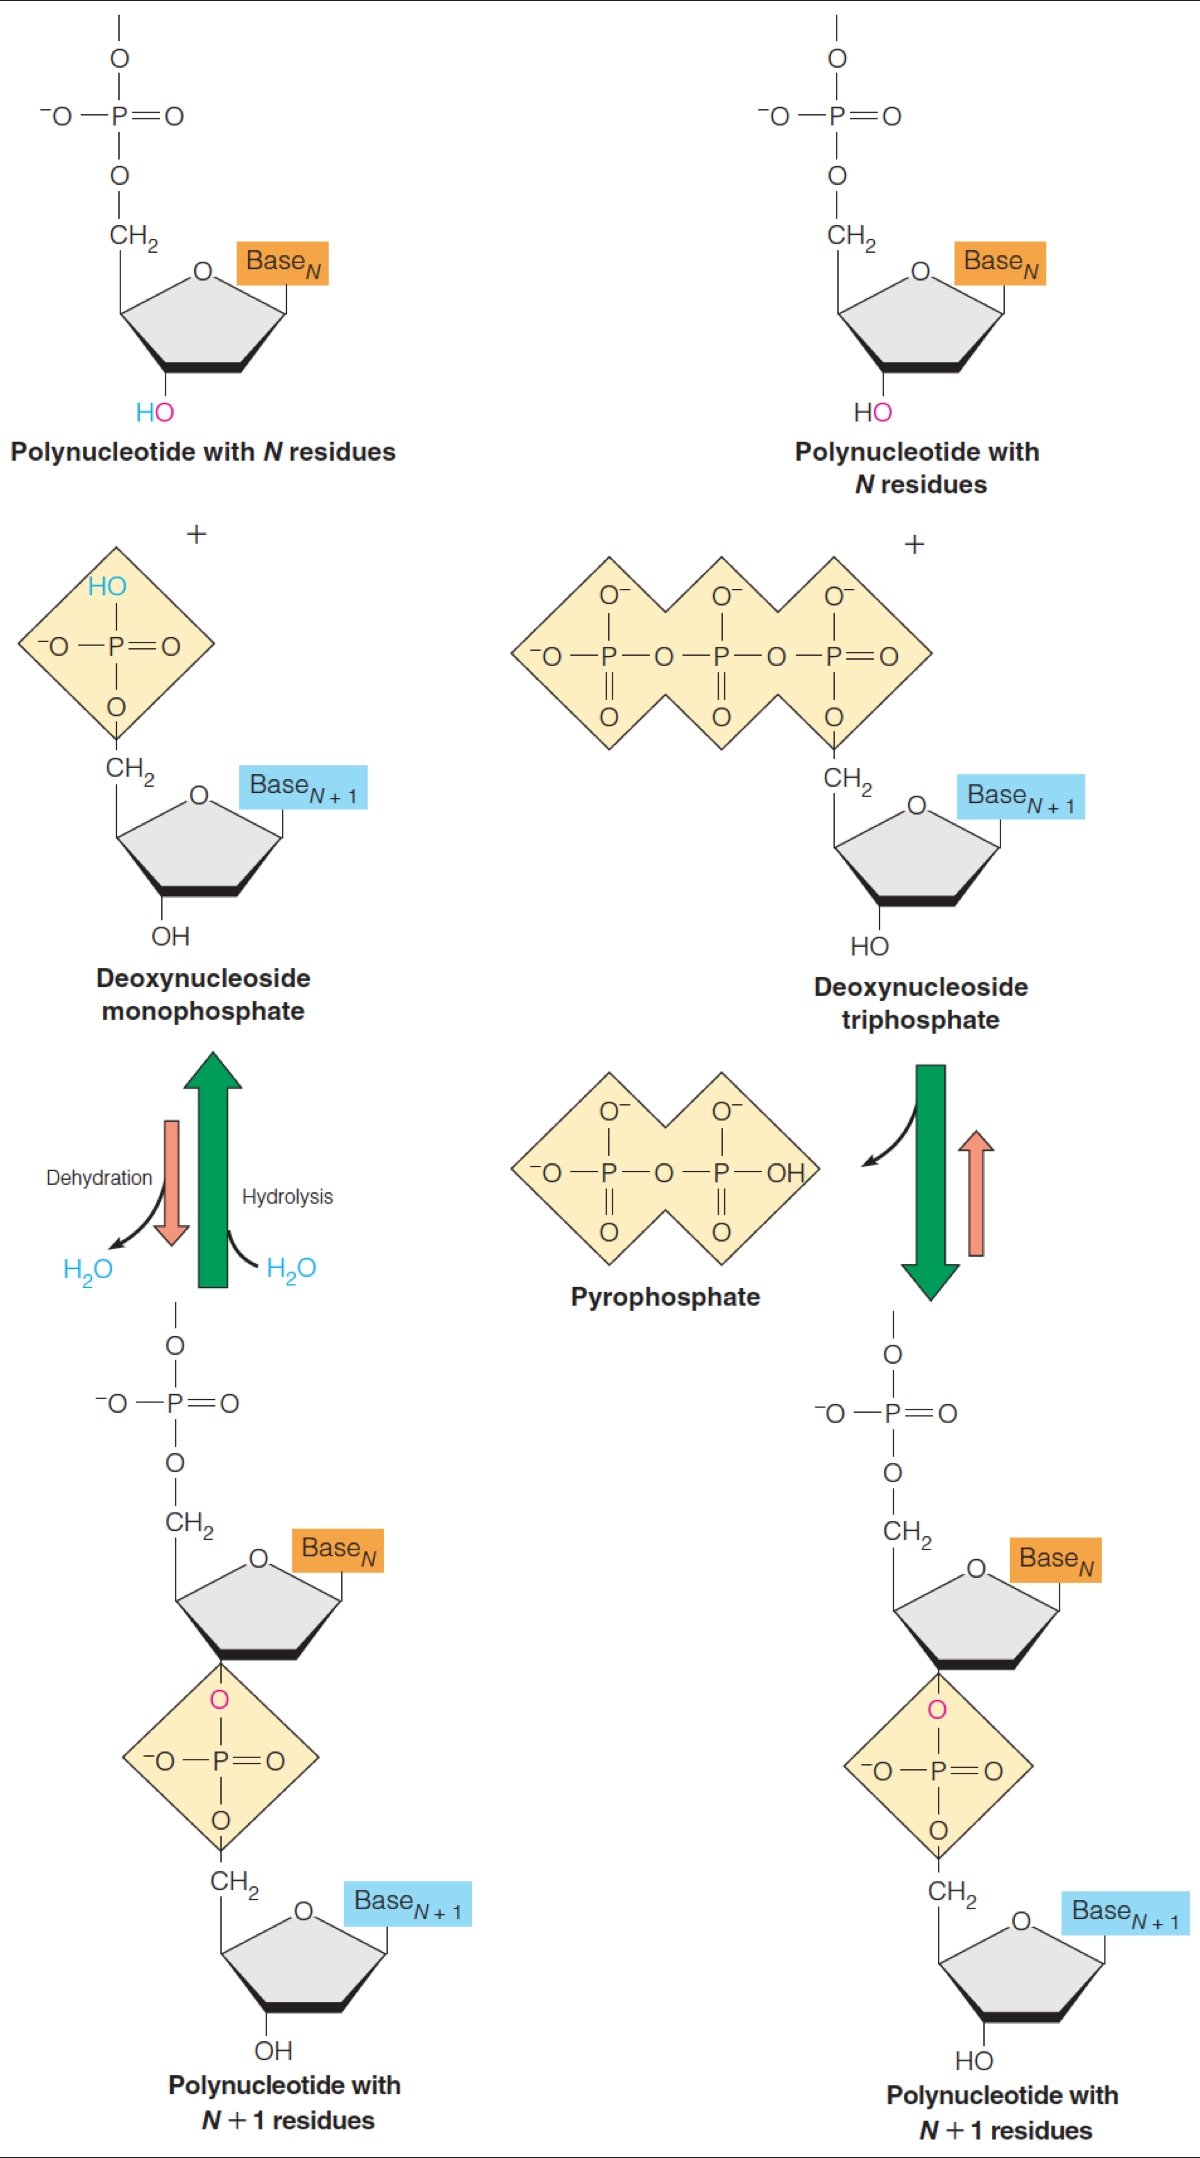
\includegraphics[width=0.9\textwidth]{NucleicAcidPolymers}
\end{figure}

\begin{itemize}
	\item Each monomer is presented as an NTP to be added to the chain.
	\begin{itemize}
		\item Prebiotic way is to dry the chemicals.
		\item In out body we split ATP, which releases energy to drive reaction.
	\end{itemize}
	\item Cleavage of the NTP provides the free energy that makes the reaction
	thermodynamically favorable.
	\item The enzymes catalyzing such reactions are
	called 	\textit{polymerases}.
	\item Mixing all of the biomolecules together in the
	appropriate ratios that living things have, does not
	create life.
	\item \textit{What is missing?}
\end{itemize}

\cite[19.S, Nucleic Acids (Summary)]{brown2009chemistry}
\section{Chemical Cycles and Chaos}

Chris Kempes

What properties and processes are “easy” to obtain
through physical dynamics alone?
\begin{itemize}
	\item Limit cycle
	\item Chaotic Dynamics
\end{itemize}


\textit{Brusselator} has this abstract set of chemical reactions.

\begin{align*}
A \rightarrow& X\\
B + X \rightarrow& Y + D\\
2X + Y \rightarrow& 3X \\
X \rightarrow& E
\end{align*}

These can be described by differential equations:

\begin{align*}
\dot X =& k_1 A - k_2 B X + k_3 X^2 Y -k_4 X\\
\dot Y =& k_2 B X -k_3 X^2 Y\text{, assuming that we hold concentrations of $A$ and $B$ constant in system.}  
\end{align*}

We can non-dimensionalize:
\begin{align*}
\dot x =& a - b x +x^2 y -x\\
\dot y =& bx - x^2 y\text{, which has steady state}\\
x^* =& a\\
y^* =& \frac{b}{a}
\end{align*}

Steady state is unstable for $b>a^2+1$. 

\begin{figure}[H]
	\caption{Brusselator Stability}\label{fig:BrusselatorStability}
	
	\begin{subfigure}[b]{0.3\textwidth}
		\centering
		\caption{ $b\ll a^2+1$}\label{fig:BrusselatorSteadyState1} 
		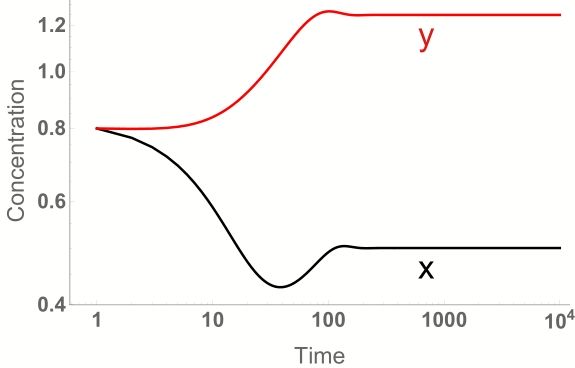
\includegraphics[width=\textwidth]{BrusselatorSteadyState1}
	\end{subfigure}
	\begin{subfigure}[b]{0.3\textwidth}
		\centering
		\caption{$b<a^2+1$, but close!}\label{fig:BrusselatorSteadyState2} 
		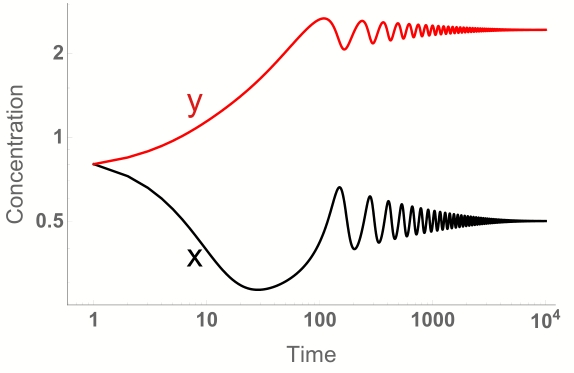
\includegraphics[width=\textwidth]{BrusselatorSteadyState2}
	\end{subfigure}
	\begin{subfigure}[b]{0.3\textwidth}
	\centering
	\caption{$b>a^2+1$}\label{fig:BrusselatorChaos} 
	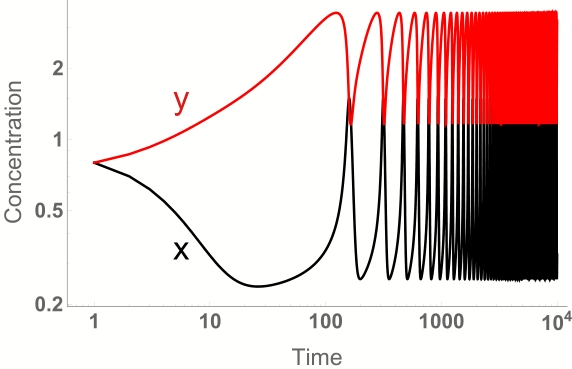
\includegraphics[width=\textwidth]{BrusselatorChaos}
\end{subfigure}
	
	
\end{figure}

See also \cite{ault2003dynamics}.


% end of text 

% glossary : may need command makeglossaries.exe origins1
\printglossaries

% bibliography goes here
 
\bibliographystyle{unsrt}
\addcontentsline{toc}{section}{Bibliography}
\bibliography{origins,wikipedia}

\end{document}
